\newpage
\section{Resultados}

\subsection{Método para sinalização digital}
\subsubsection{Estabelecendo a geração de dados}
    Foi montado o módulo U-2970A de acordo com o roteiro, como mostra a figura \ref{fig:r1a}.
    A saída obtida no osciloscópio se encontra na figura \ref{fig:r1a-2}.
    
            \begin{figure}[H]
                \centering
                \caption{Montagem parte 1.}
                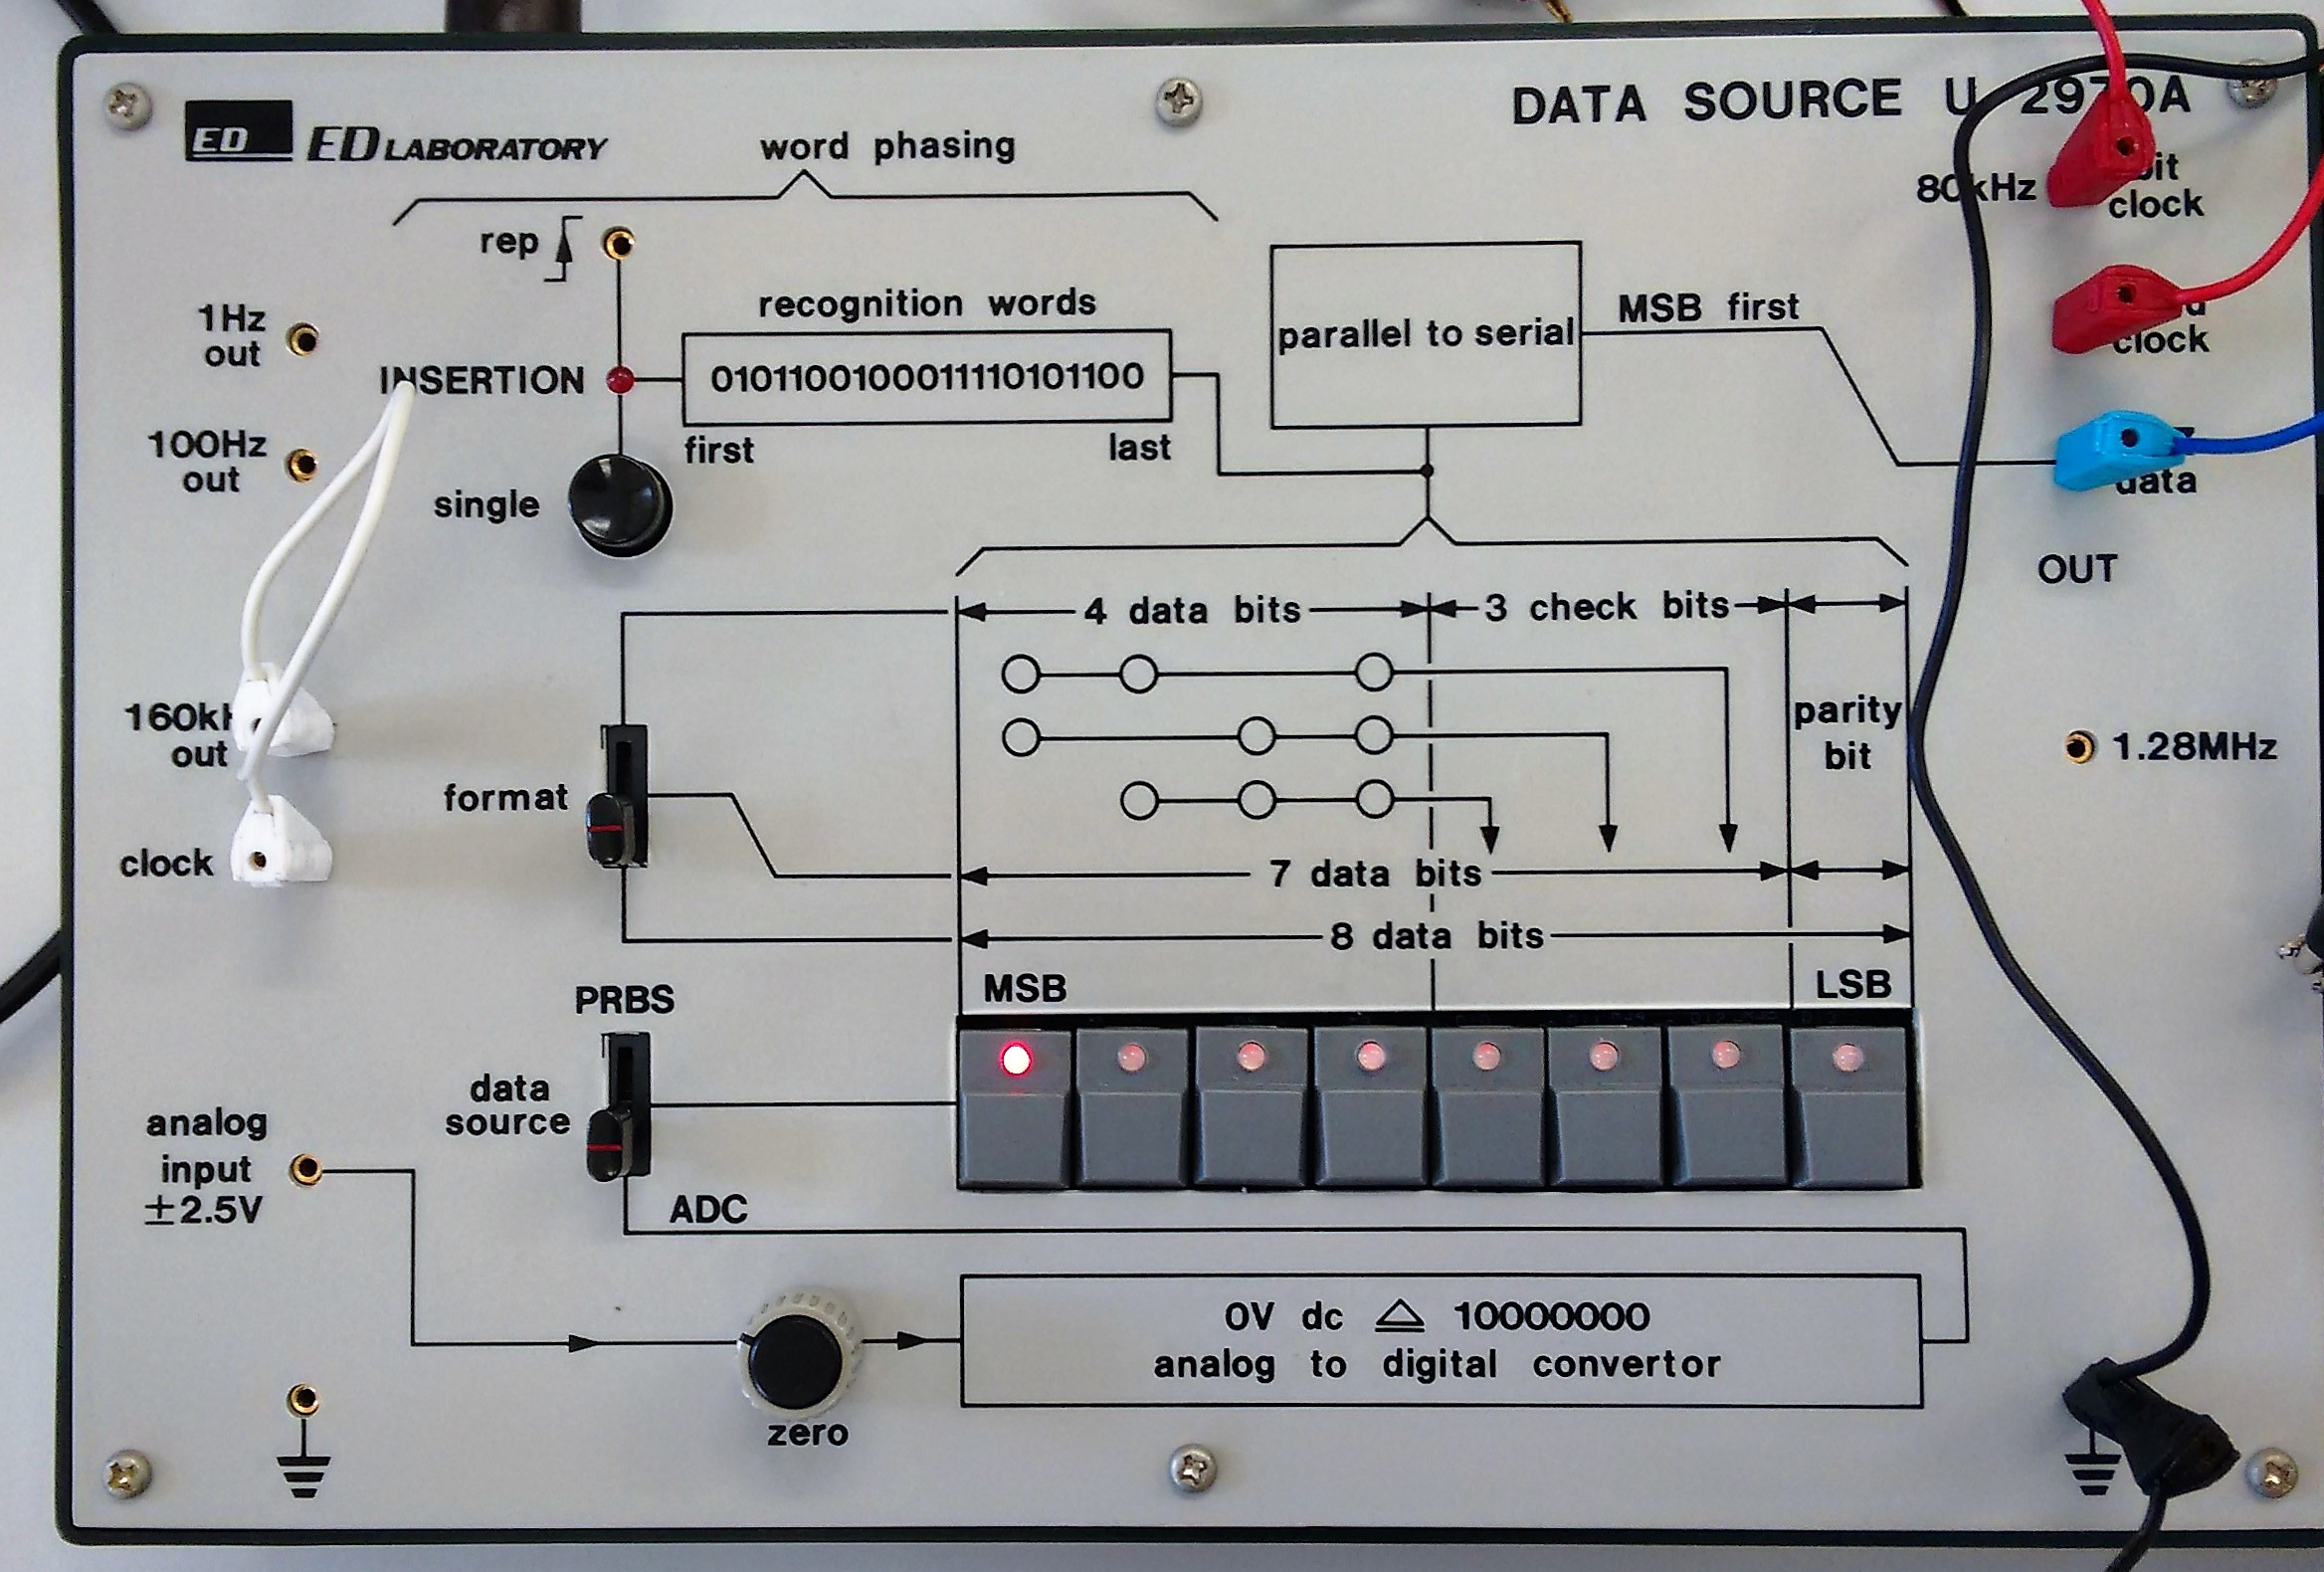
\includegraphics[scale=0.1]{r1a}
                
                \label{fig:r1a}
            \end{figure}
            
            \begin{figure}[H]
                \centering
                \caption{Saída parte 1.}
                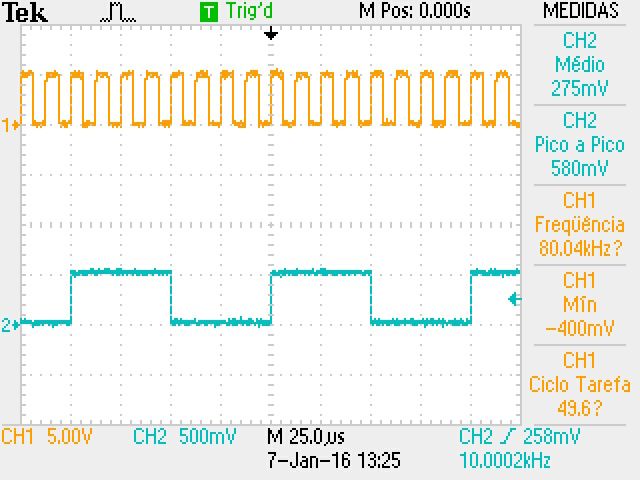
\includegraphics[scale=0.3]{r1a-2}
                
                \label{fig:r1a-2}
            \end{figure}

    \subsubsection{Enviando um sinal analógico e digitalizando-o}
    Foi montado o módulo U-2970A de acordo com o roteiro, como mostra a figura \ref{fig:r2a}.
            \begin{figure}[H]
                \centering
                \caption{Montagem parte 2.}
                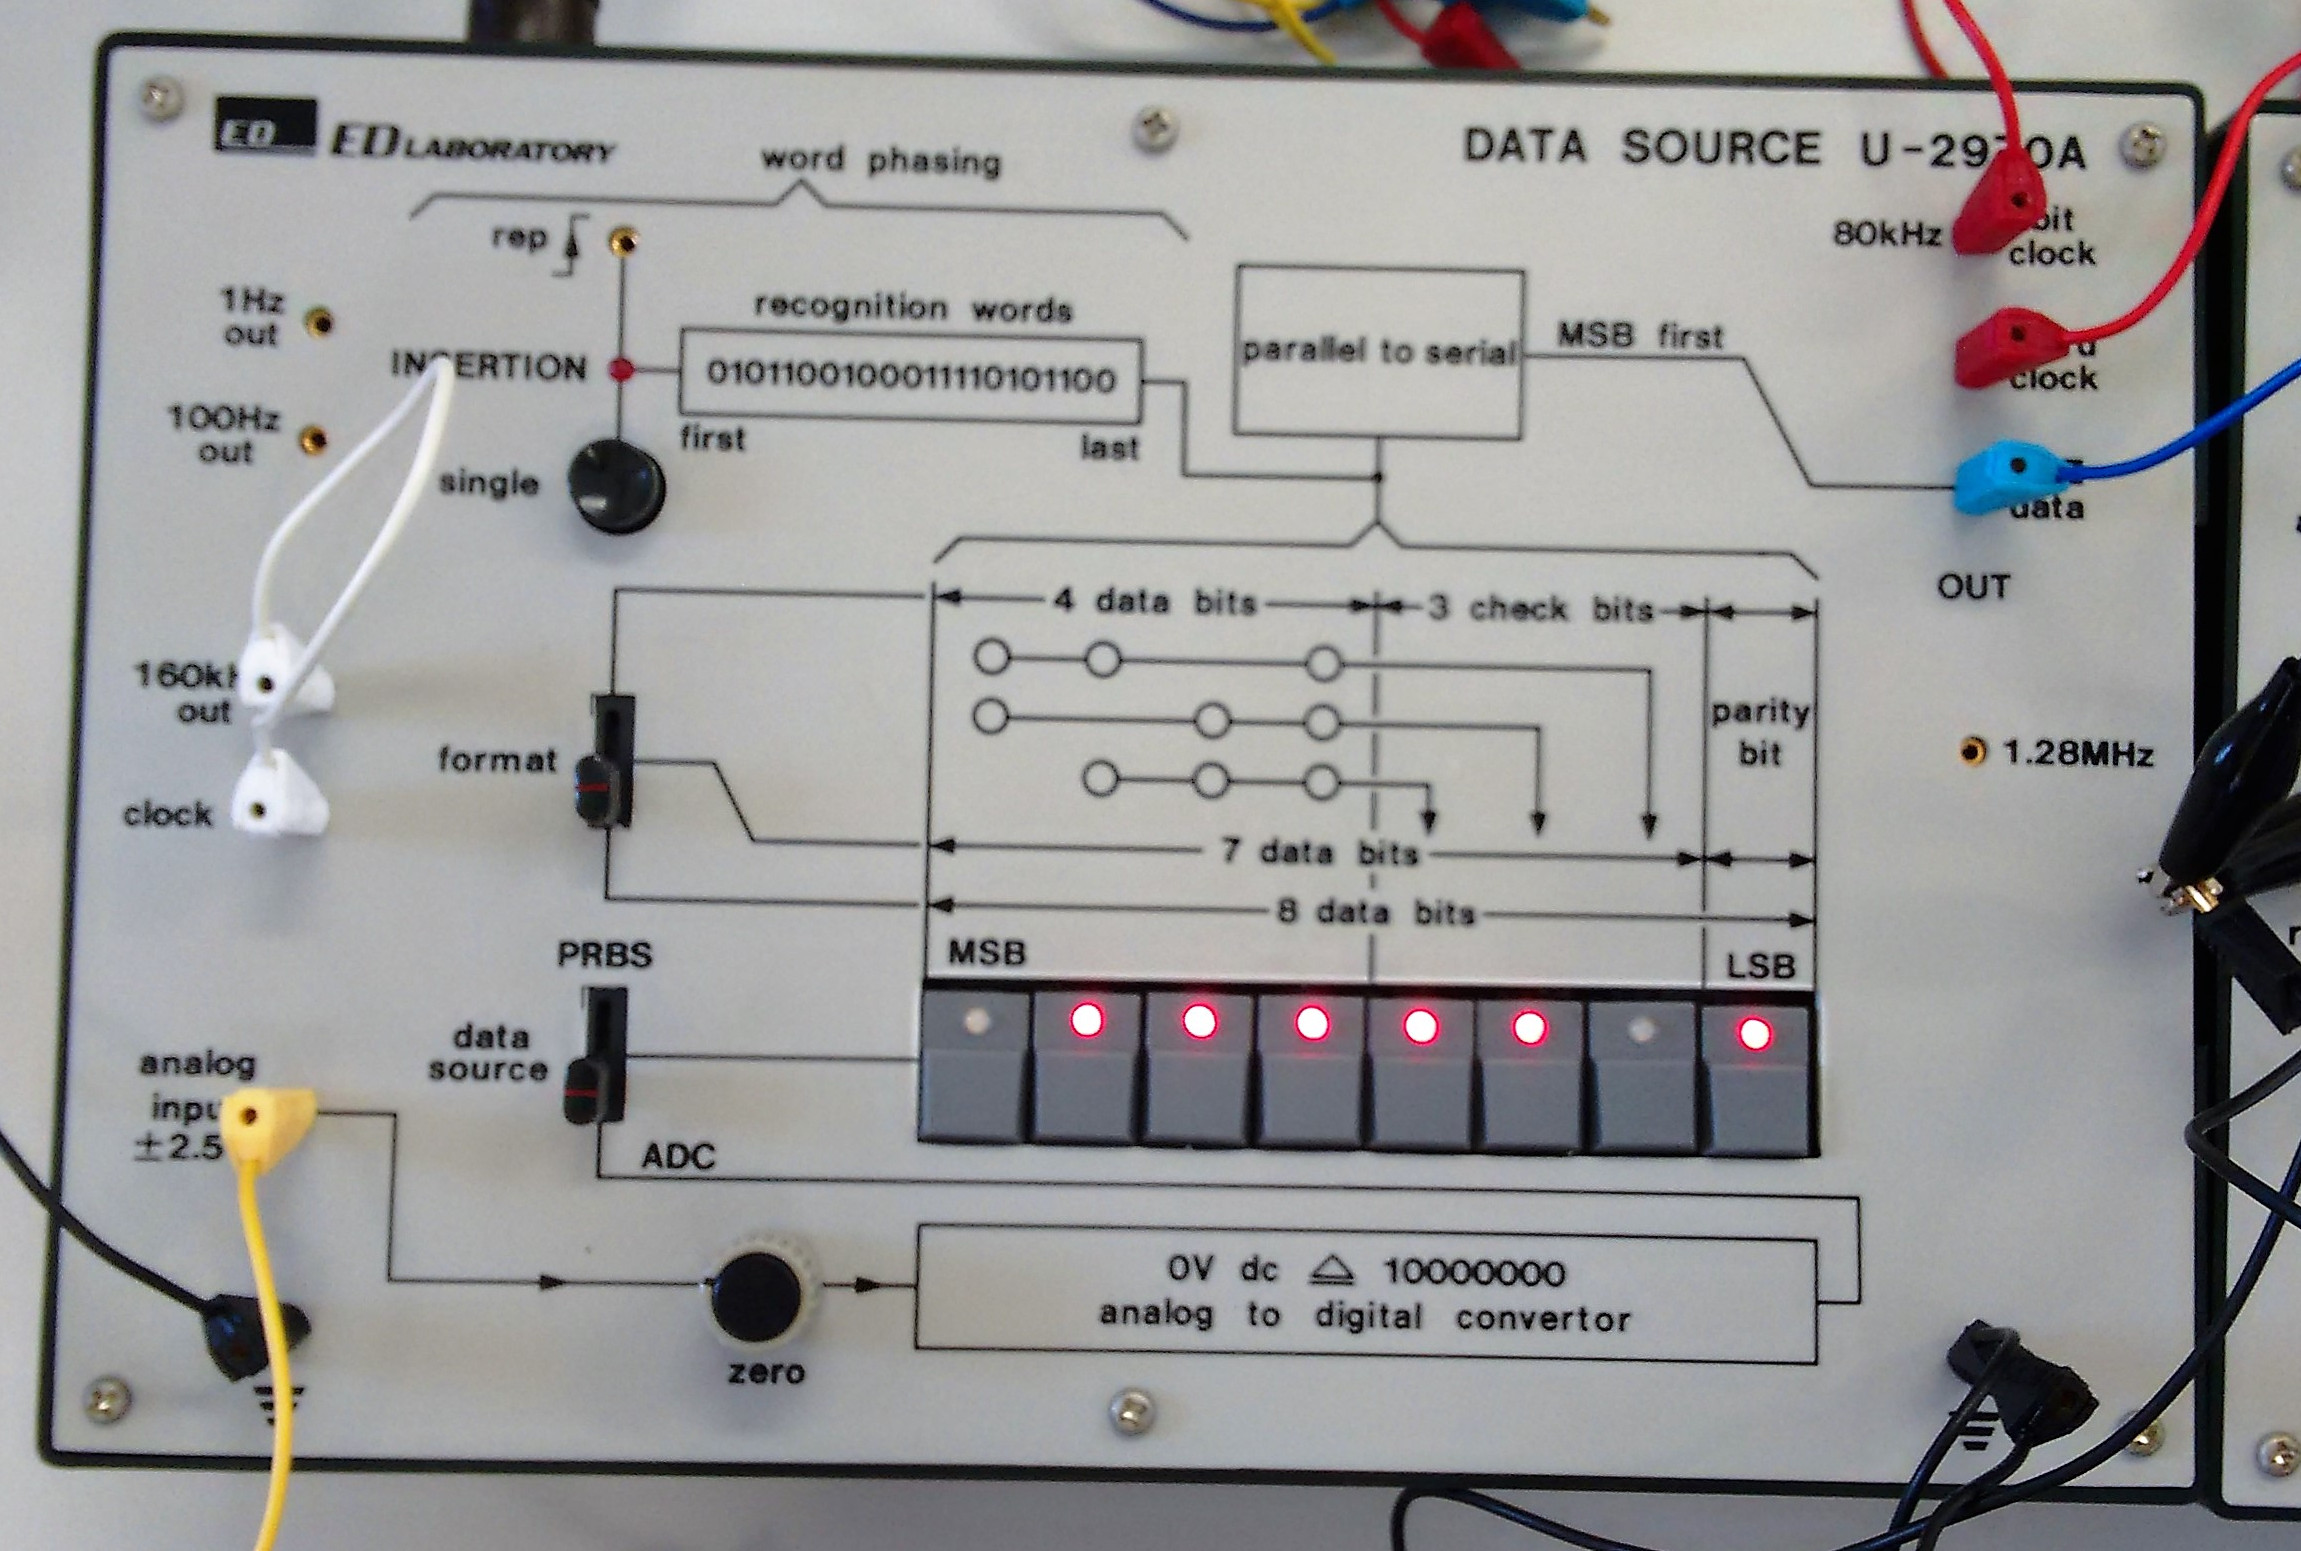
\includegraphics[scale=0.1]{r2a}
                
                \label{fig:r2a}
            \end{figure}

            
    \subsubsection{Recebendo Palavras Códigos}
     Foi montado o módulo U-2970A de acordo com o roteiro, como mostra a figura \ref{fig:r3a}.
     A saída obtida no osciloscópio se encontra na figura \ref{fig:r3a-2}.
     \begin{figure}[H]
         \centering
         \caption{Montagem parte 3.}
         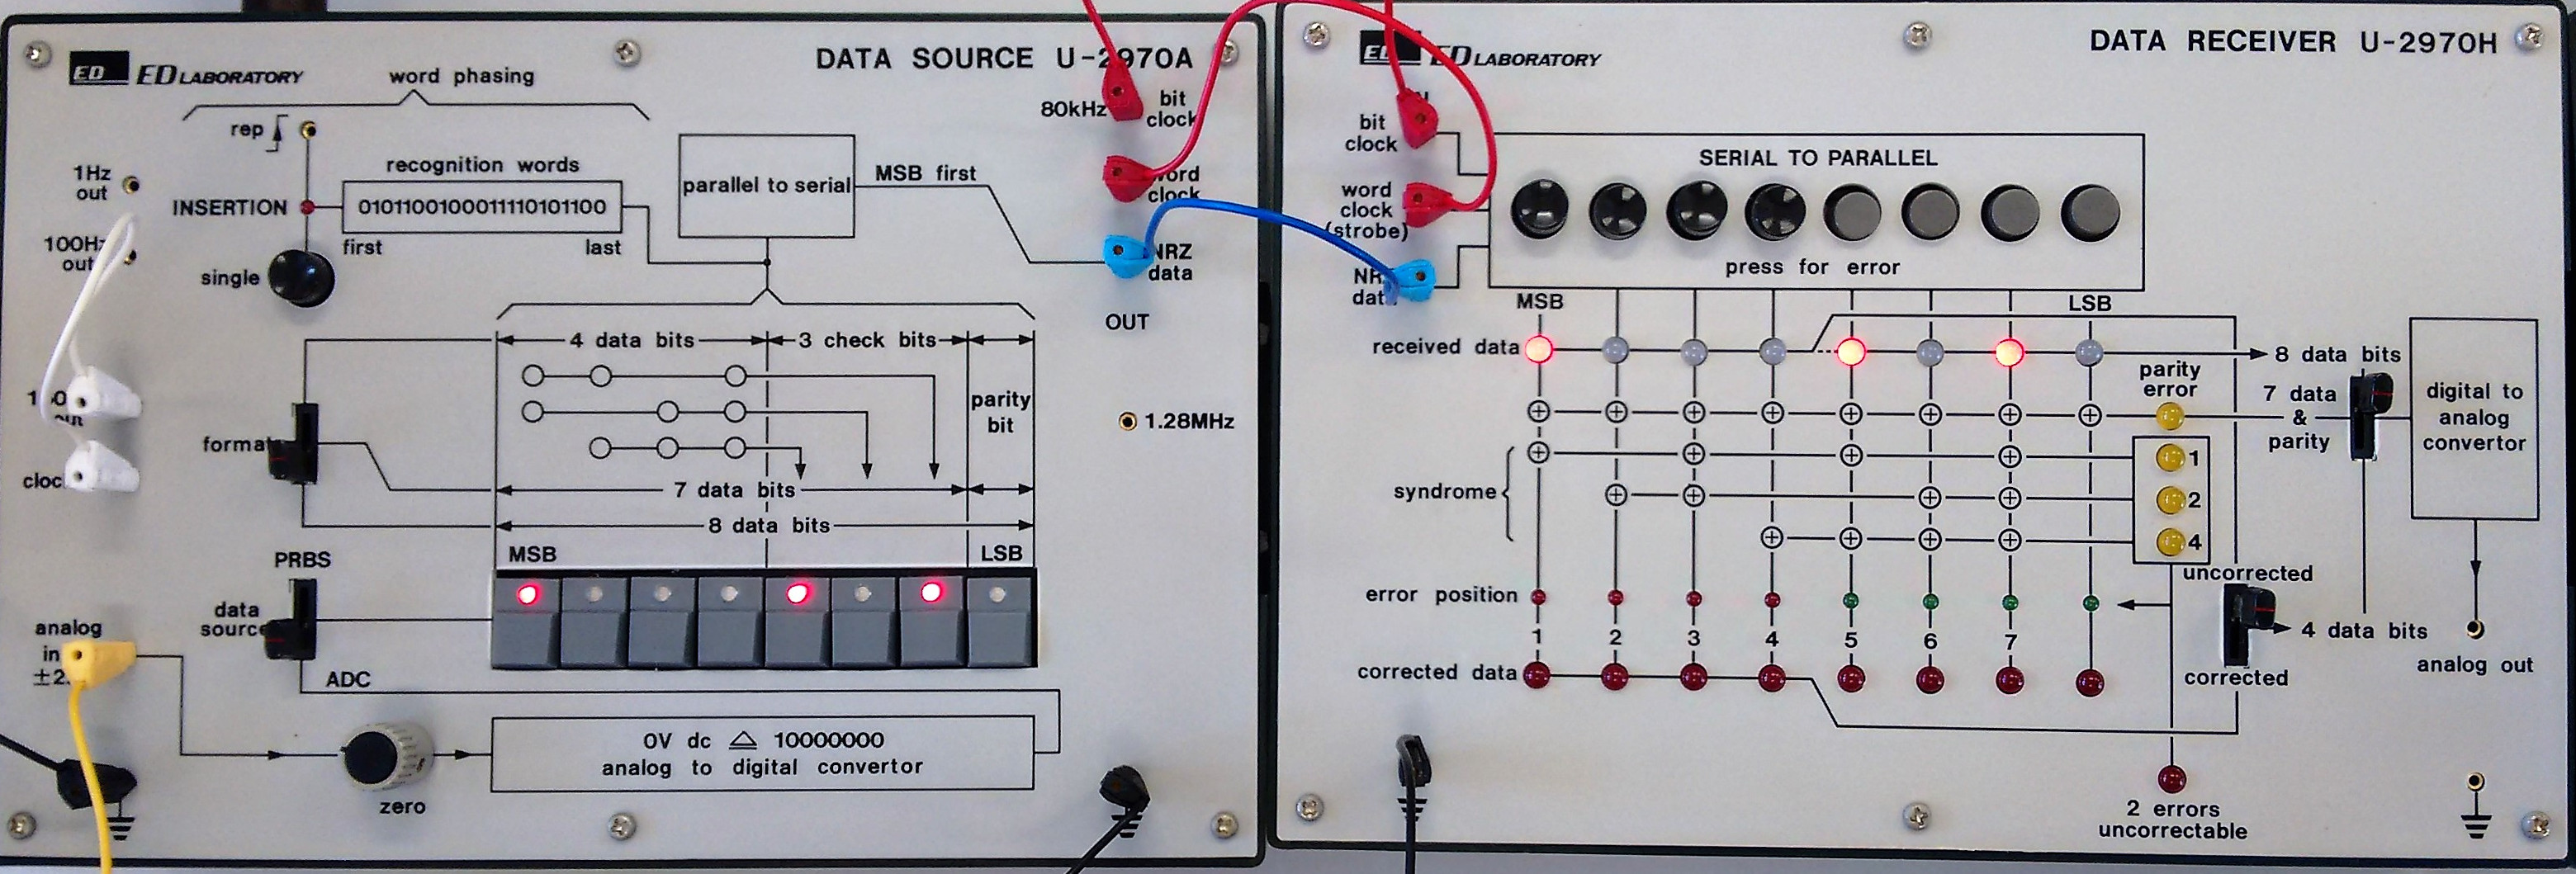
\includegraphics[scale=0.1]{r3a}
         
         \label{fig:r3a}
        \end{figure}
            
        \begin{figure}[H]
            \centering
            \caption{Saída parte 3.}
            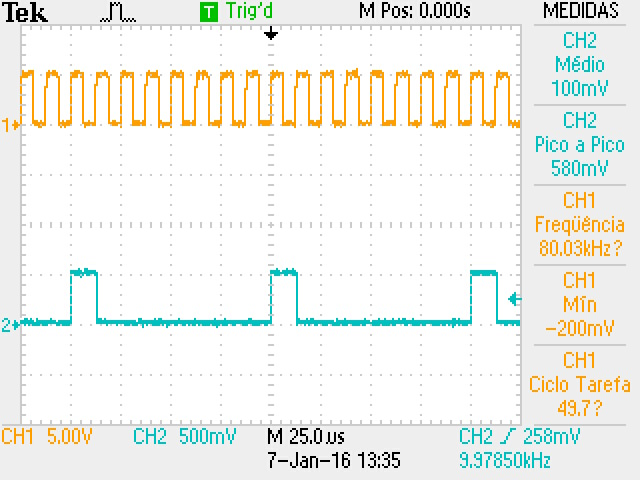
\includegraphics[scale=0.3]{r3a-2}
            
            \label{fig:r3a-2}
        \end{figure}

    \subsubsection{Obtendo Saída Analógica}
    A montagem foi feita como mostra a figura \ref{fig:r4a}. A saída obtida se encontra na figura \ref{fig:r4a-2}.
    
         \begin{figure}[H]
             \centering
             \caption{Montagem parte 4.}
             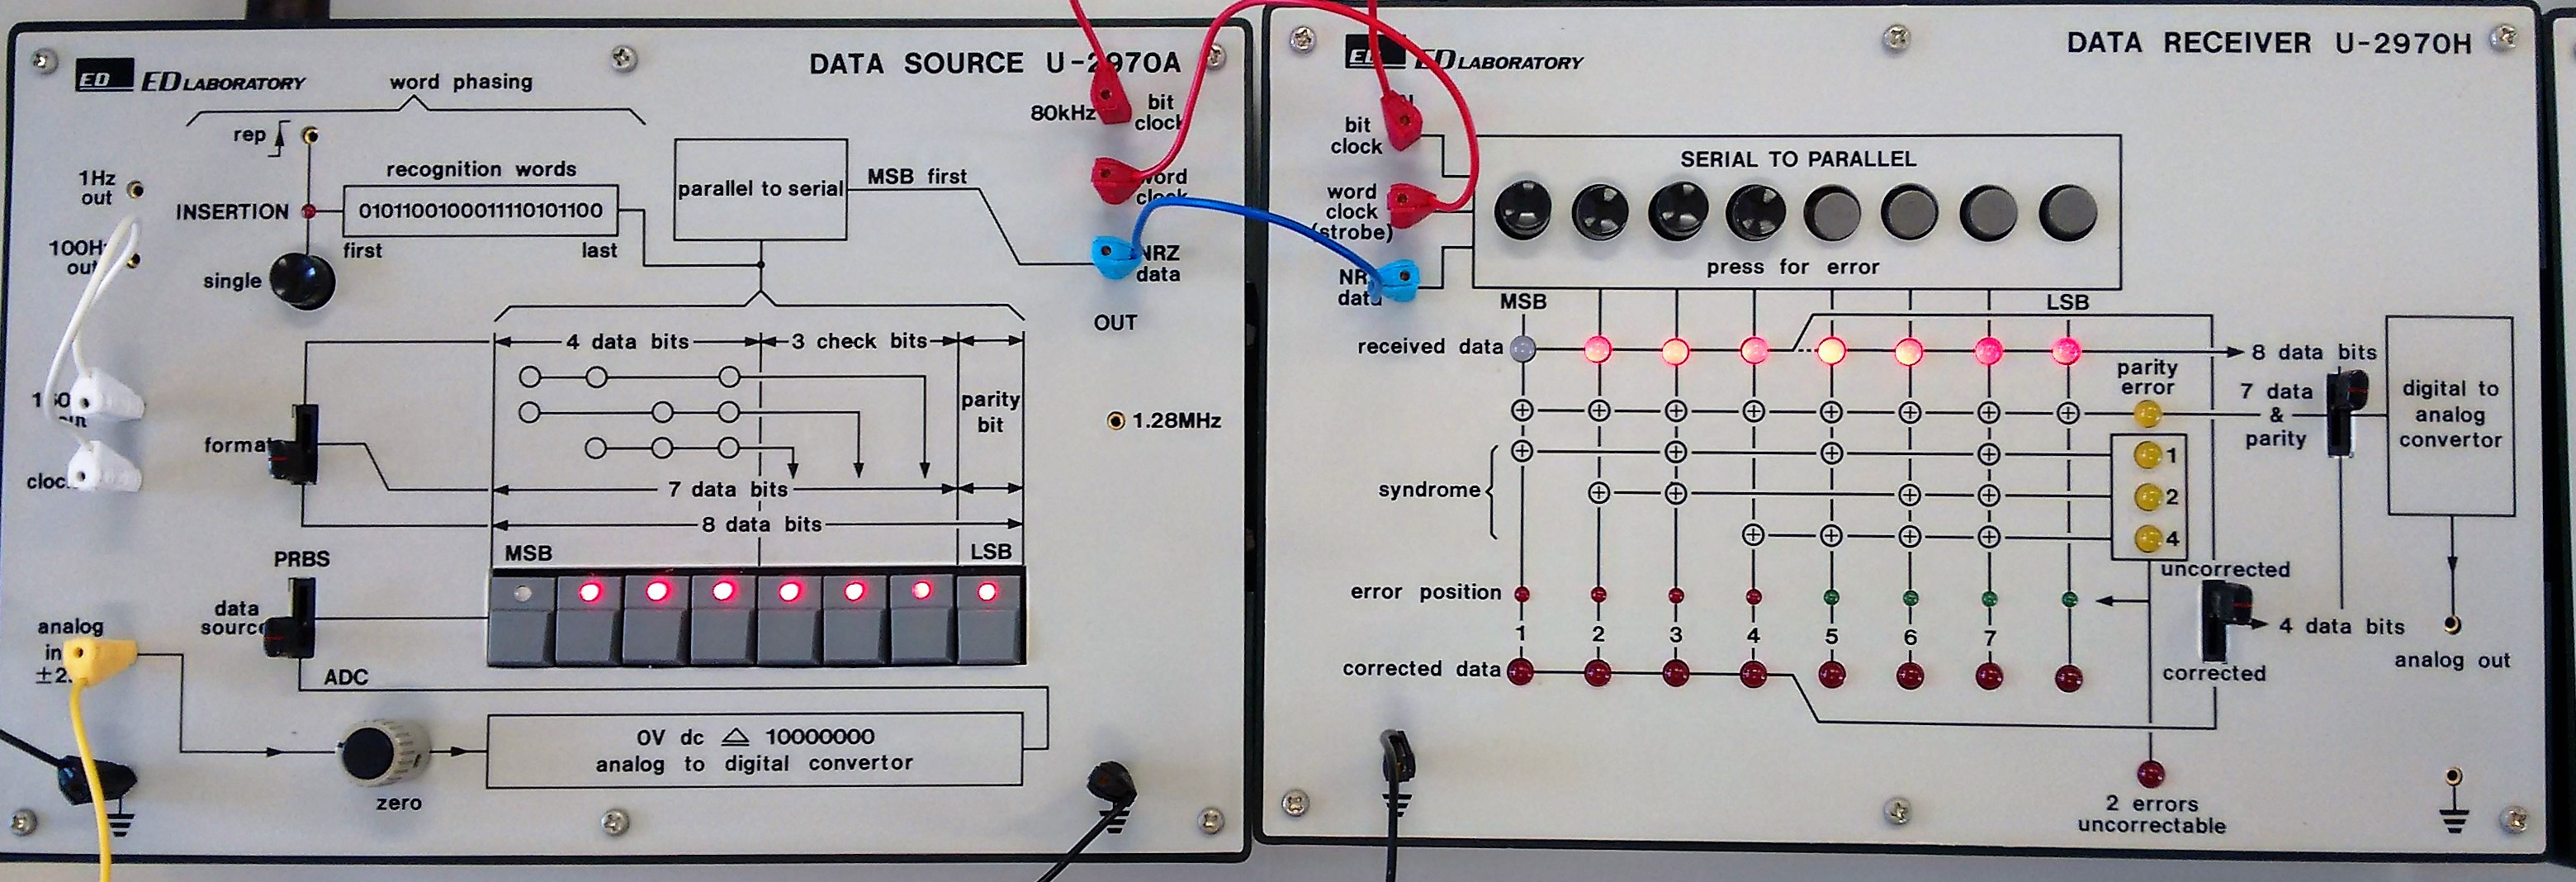
\includegraphics[scale=0.1]{r4a}
             
             \label{fig:r4a}
            \end{figure}
            
            \begin{figure}[H]
                \centering
                \caption{Saída parte 4.}
                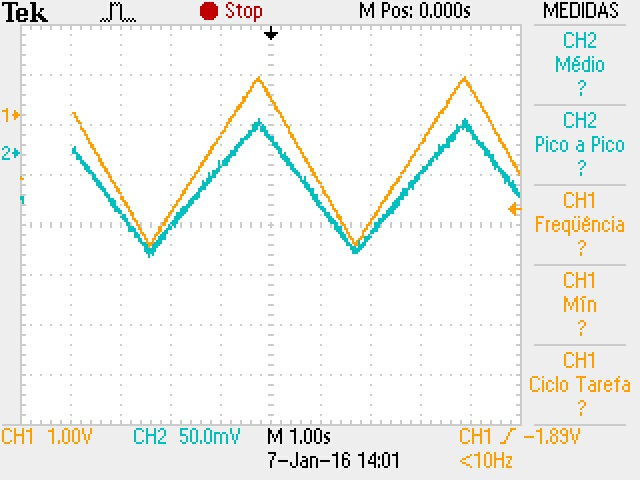
\includegraphics[scale=0.3]{r4a-2}
                
                \label{fig:r4a-2}
            \end{figure}
            
   \subsubsection{Operando o Módulo de Áudio U-2970K}
    A montagem foi feita como mostra a figura \ref{fig:r5a}. O resultado é que foi possível ouvir claramente a onda senoidal de 600Hz na saída do módulo U-2970K.
     
     \begin{figure}[H]
         \centering
         \caption{Montagem parte 5.}
         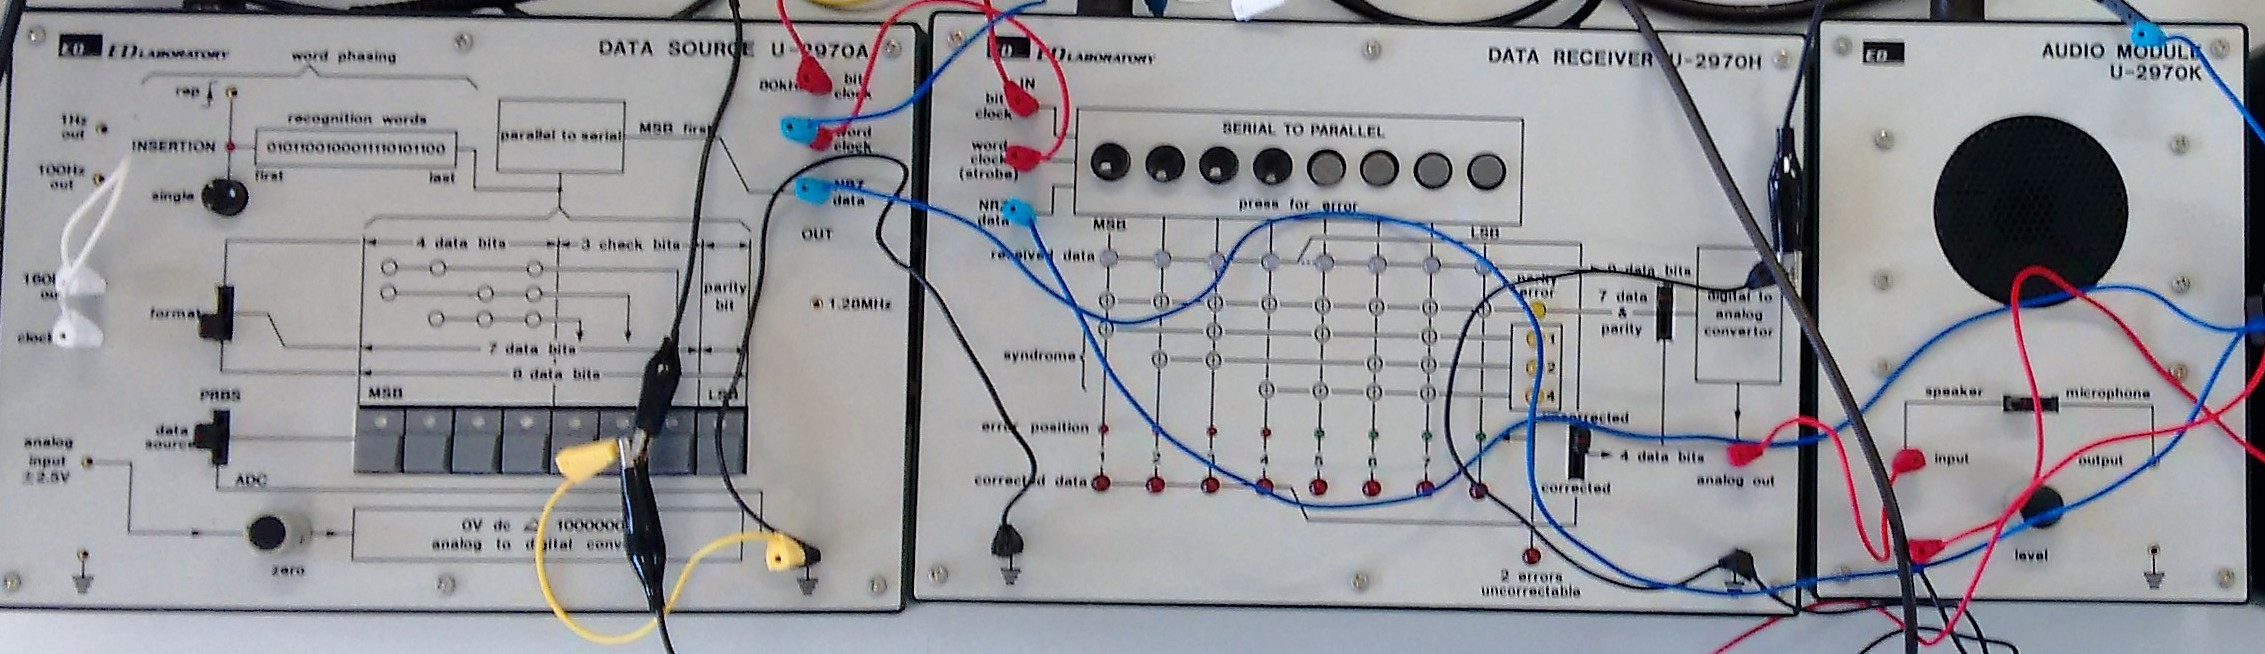
\includegraphics[scale=0.2]{r5a}
         
         \label{fig:r5a}
        \end{figure}
        
    \subsubsection{Completando o Canal Digital de Áudio}
    Nessa parte foi observado que para frequências acima de 5kHz o som apresentou distorções. Isso foi causado pelo critério de Nyquist, que determina que a taxa de amostragem dever ser no mínimo duas vezes maior que a largura de banda do sinal. Como o ADC utilizado possui frequência de amostragem de 10kHz, a frequência máxima a ser transmitida deve ser menor que 5kHz, caso contrário há degradação do sinal, como foi observado.
    
    \subsubsection{Testando um Telefone Simples}
        Como não havia um segundo módulo de áudio disponível, foi utilizado o gerador de funções para gerar um ruído. Foi possível escutar um chiado, porém, o mesmo era bastante diferente do fenômeno esperado (microfonia).
        
        \subsection{Ruído}
        \subsubsection{Rejeição do seu próprio ruído}
         A montagem foi feita como mostra a figura \ref{fig:r8a}.
         
              \begin{figure}[H]
                  \centering
                  \caption{Montagem parte 8.}
                  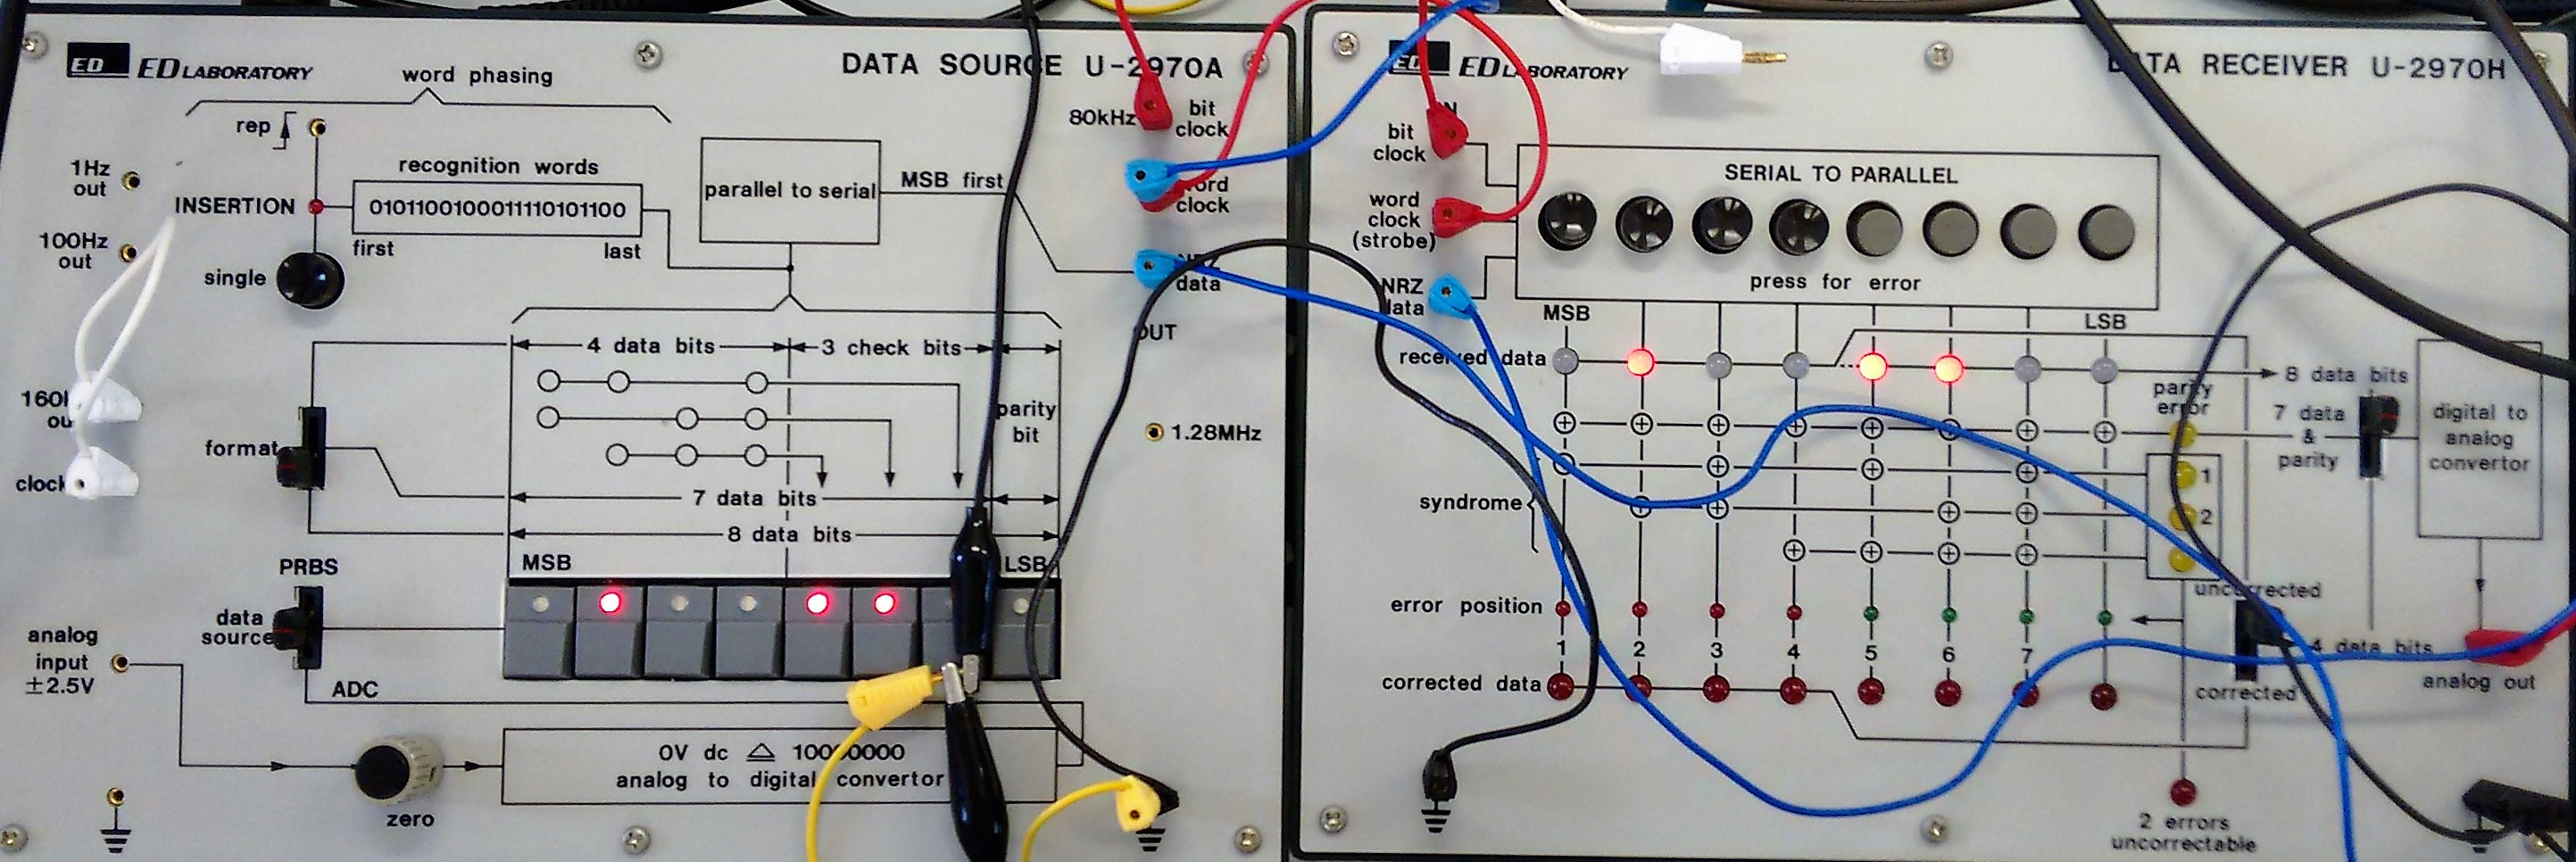
\includegraphics[scale=0.1]{r8a}
                  
                  \label{fig:r8a}
                \end{figure}
                
       Conforme previsto no roteiro, os leds ficaram todos acesos, conforme mostra a figura \ref{fig:r8a-2}.
     \begin{figure}[H]
         \centering
         \caption{Estado da parte 8.}
         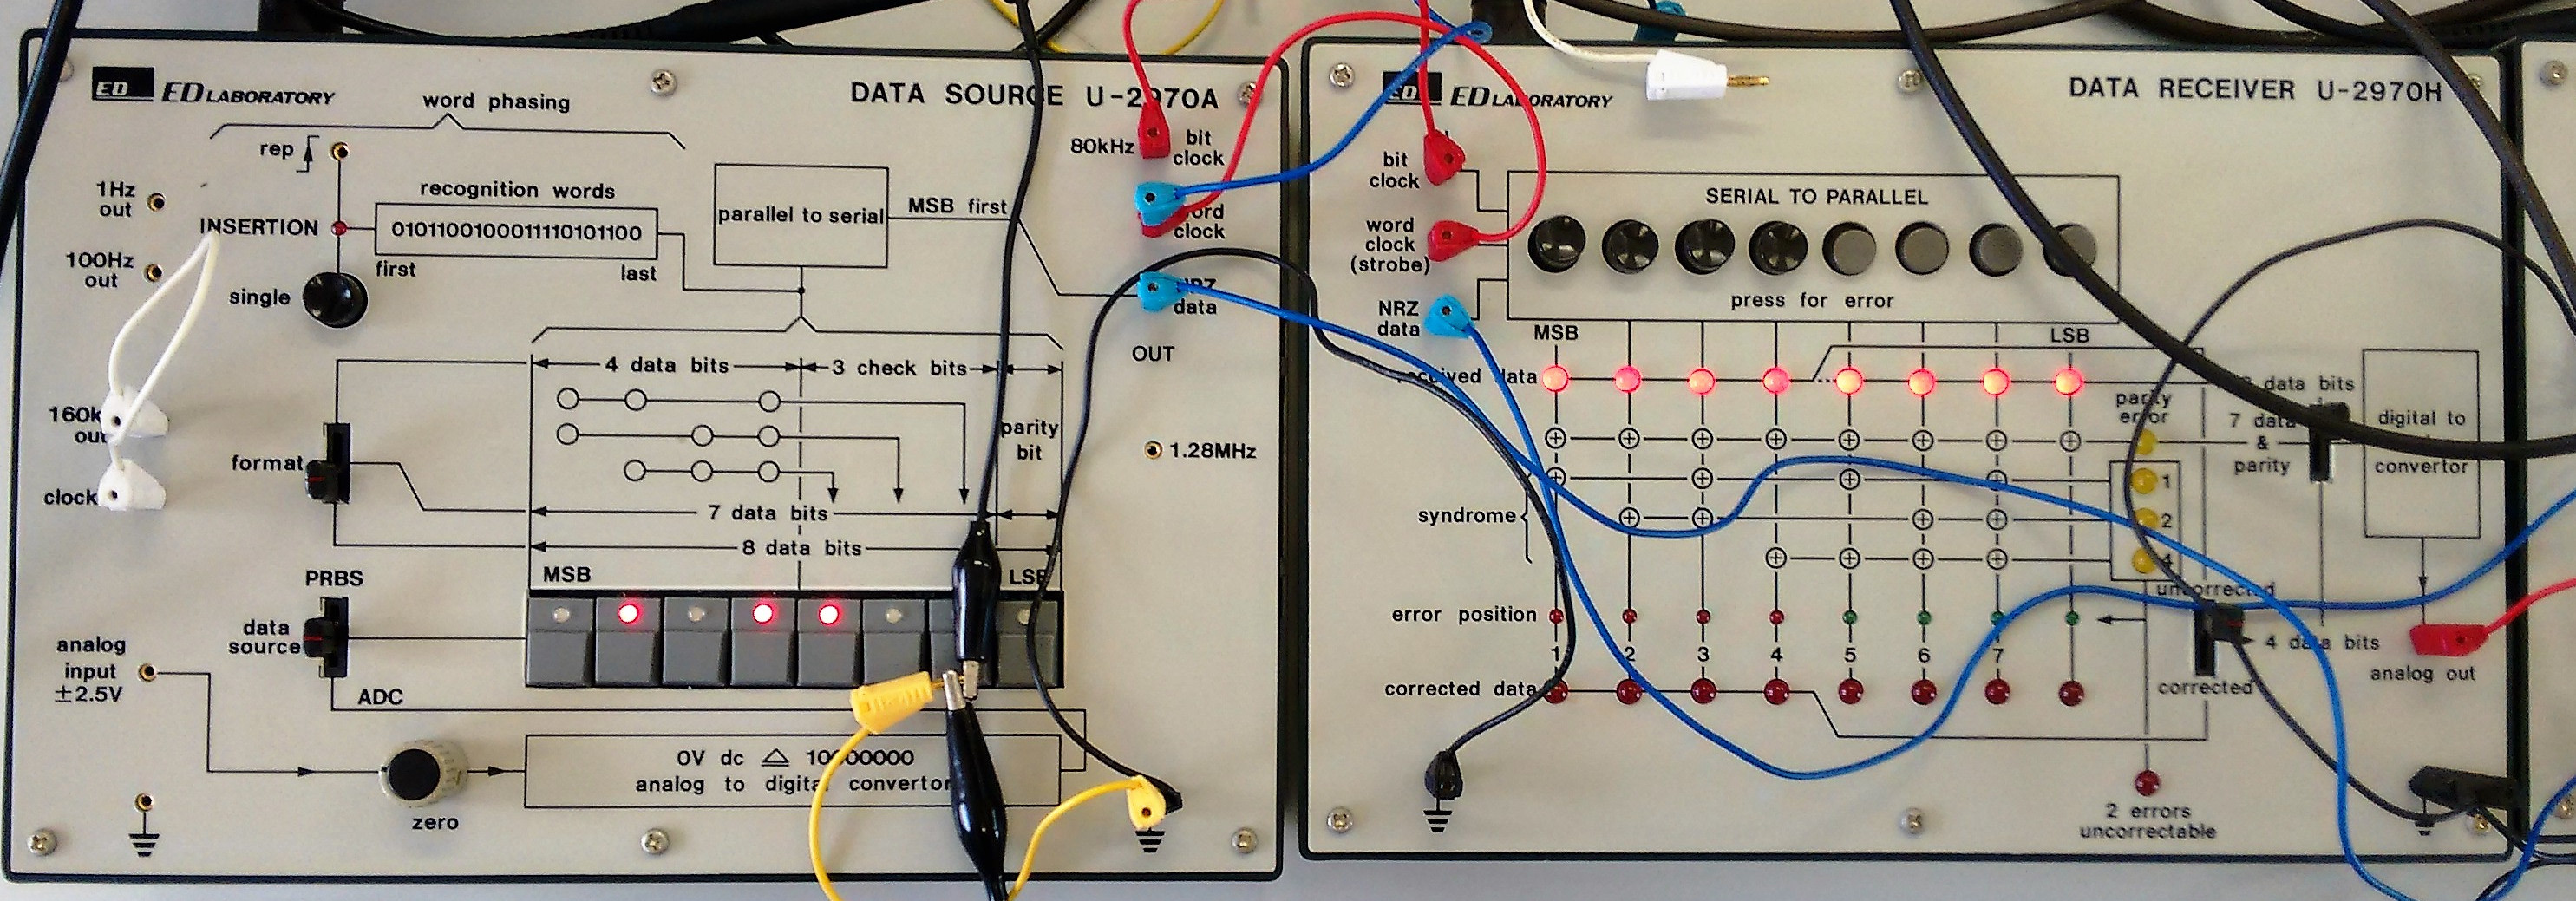
\includegraphics[scale=0.1]{r8a-2}
         
         \label{fig:r8a-2}
        \end{figure}
        
        A figura \ref{fig:r8a-3} mostra a saída no osciloscópio.
        
    \begin{figure}[H]
        \centering
        \caption{Saída parte 8.}
        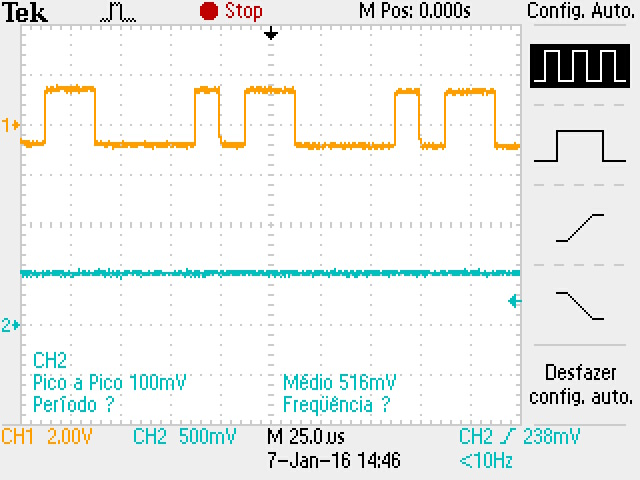
\includegraphics[scale=0.3]{r8a-3}
        
        \label{fig:r8a-3}
     \end{figure}   
     
     \subsection{Detecção e correção de erros}
     \subsubsection{Verificando a Paridade}
     
     De acordo com a imagem \ref{fig:r9a}, foi possível observar que o simbolo estava com erro, devido ao bit de paridade.
     
     
         \begin{figure}[H]
             \centering
             \caption{Saída parte 9.}
             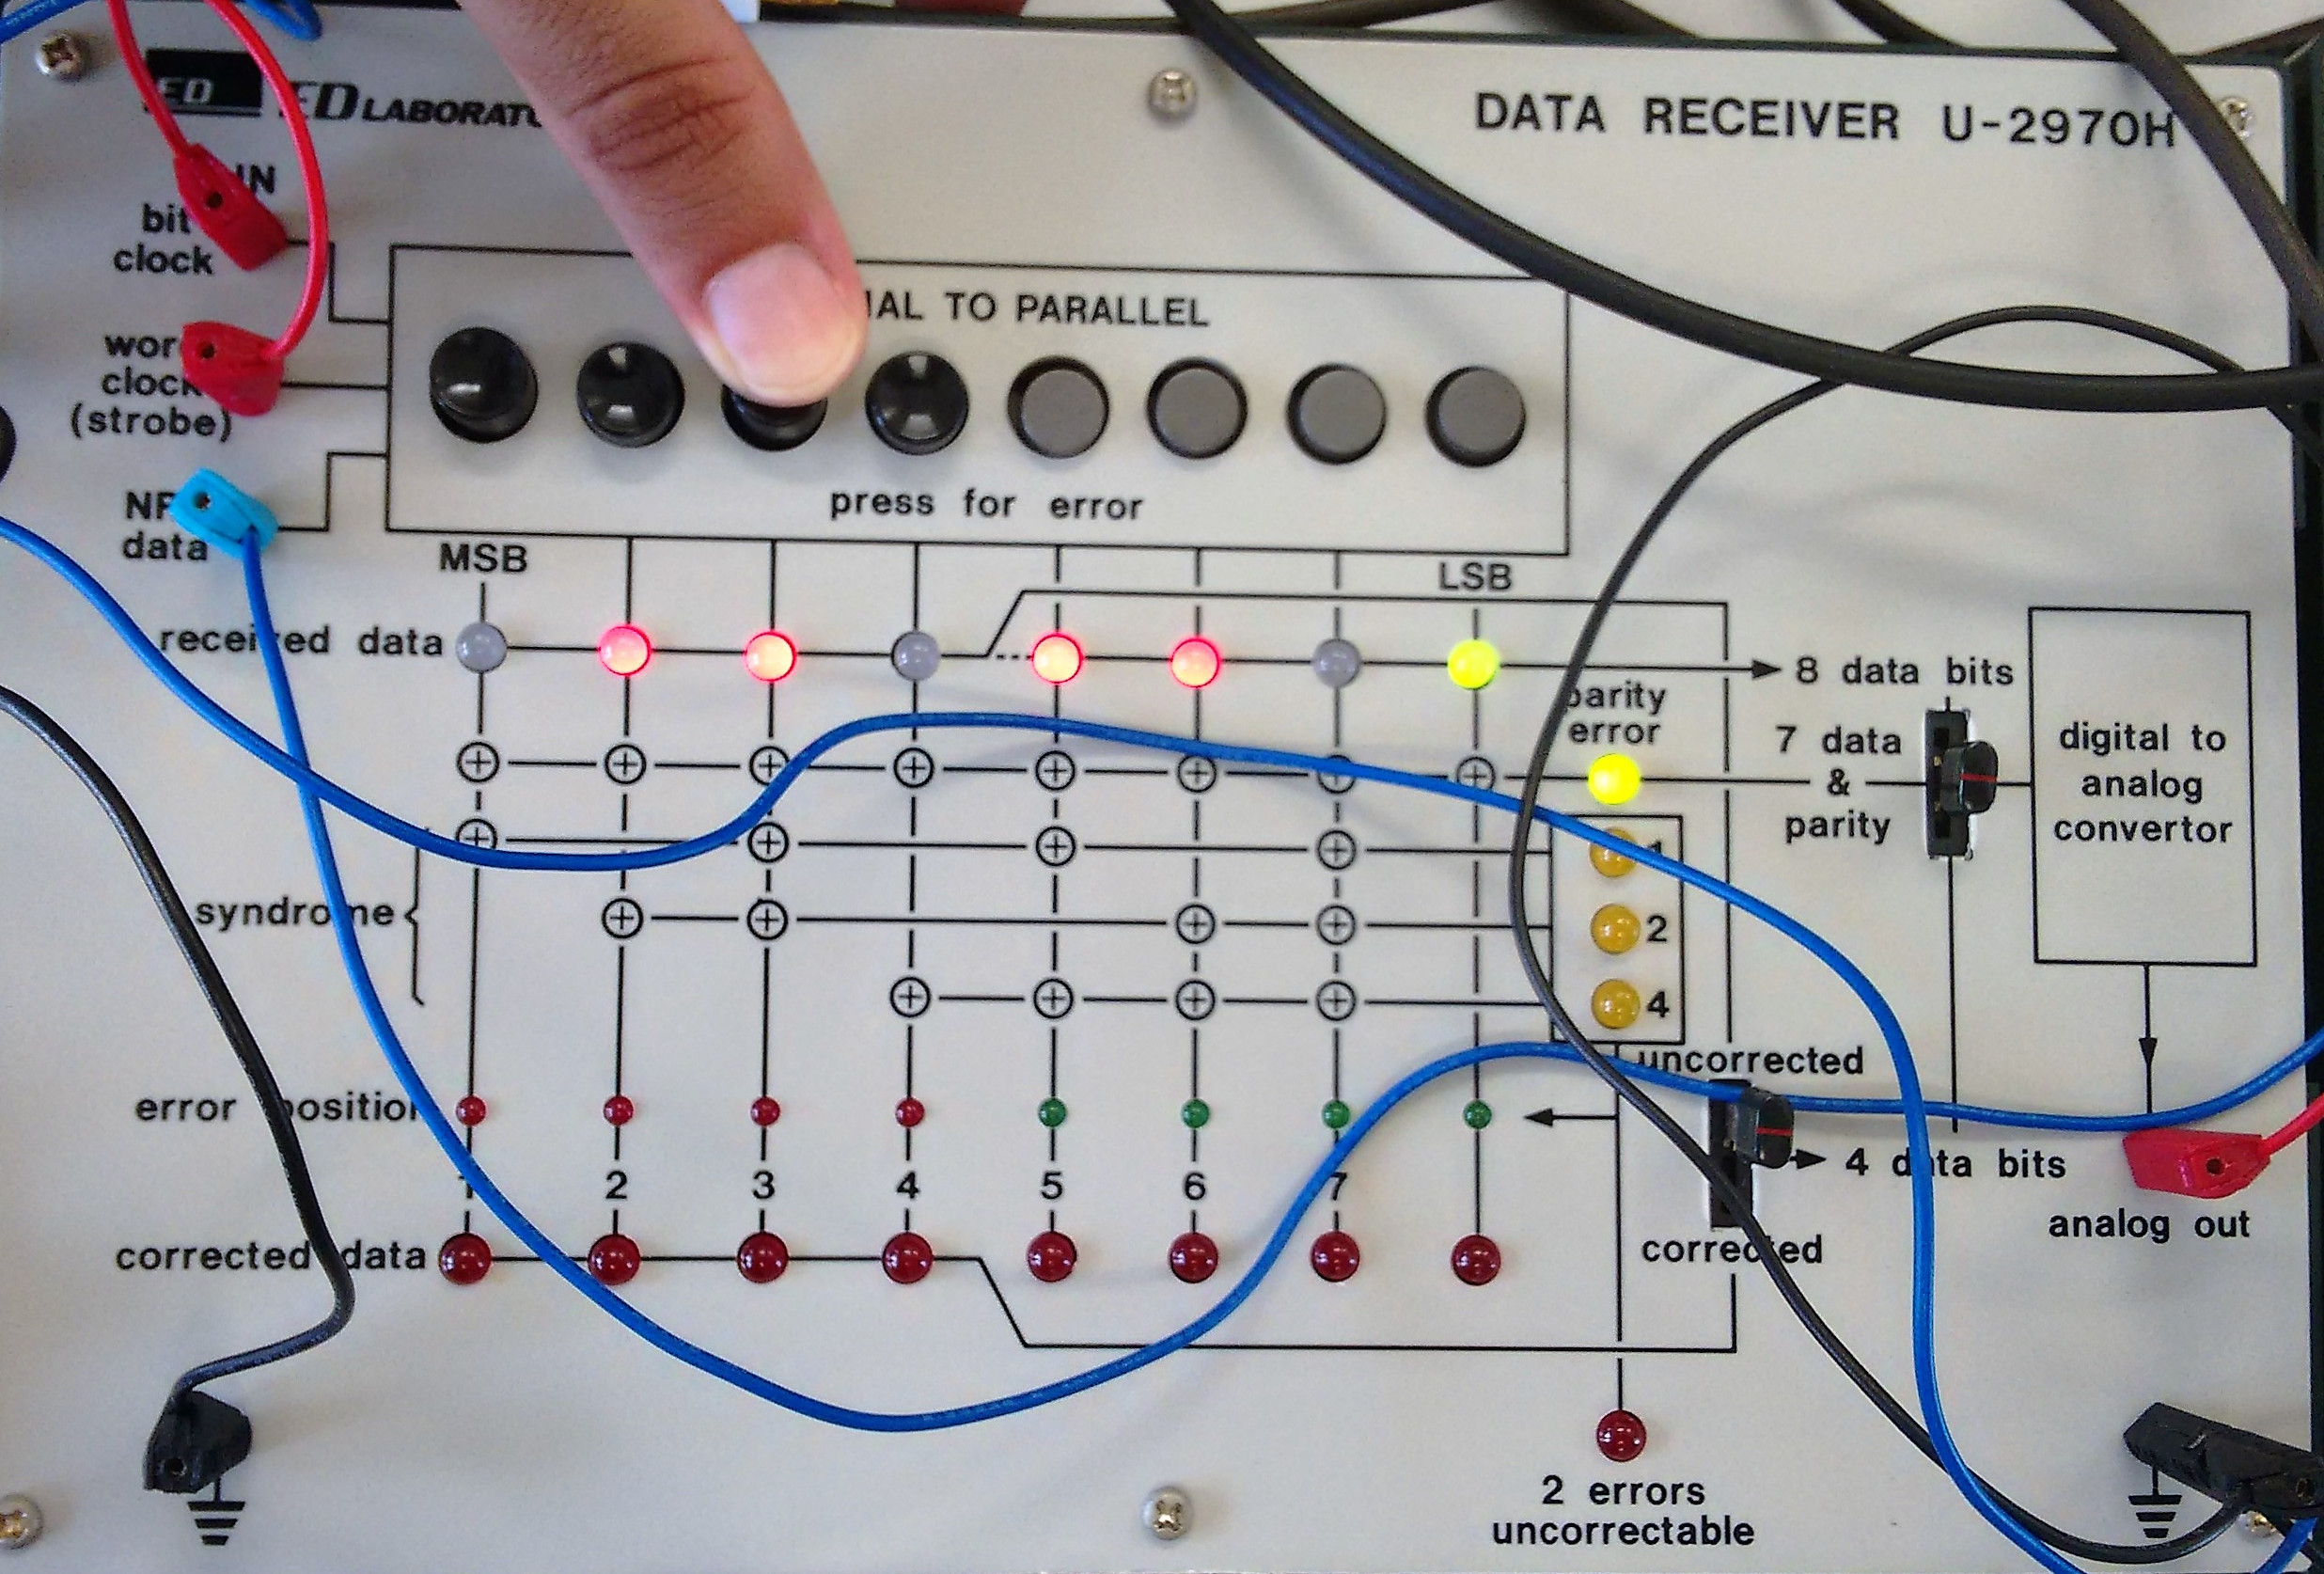
\includegraphics[scale=0.1]{r9a}
             
             \label{fig:r9a}
            \end{figure}  
            
     \subsubsection{Correção do erro} 
     A montagem foi feita e, conforme esperado, o bit de erro foi detectado evidenciado (conforme mostra a figura \ref{fig:r10a}).
     Notou-se que para apenas 1 bit de erro, o sinal com correção não apresenta mudanças na saída.
     
     \begin{figure}[H]
         \centering
         \caption{Saída parte 10.}
         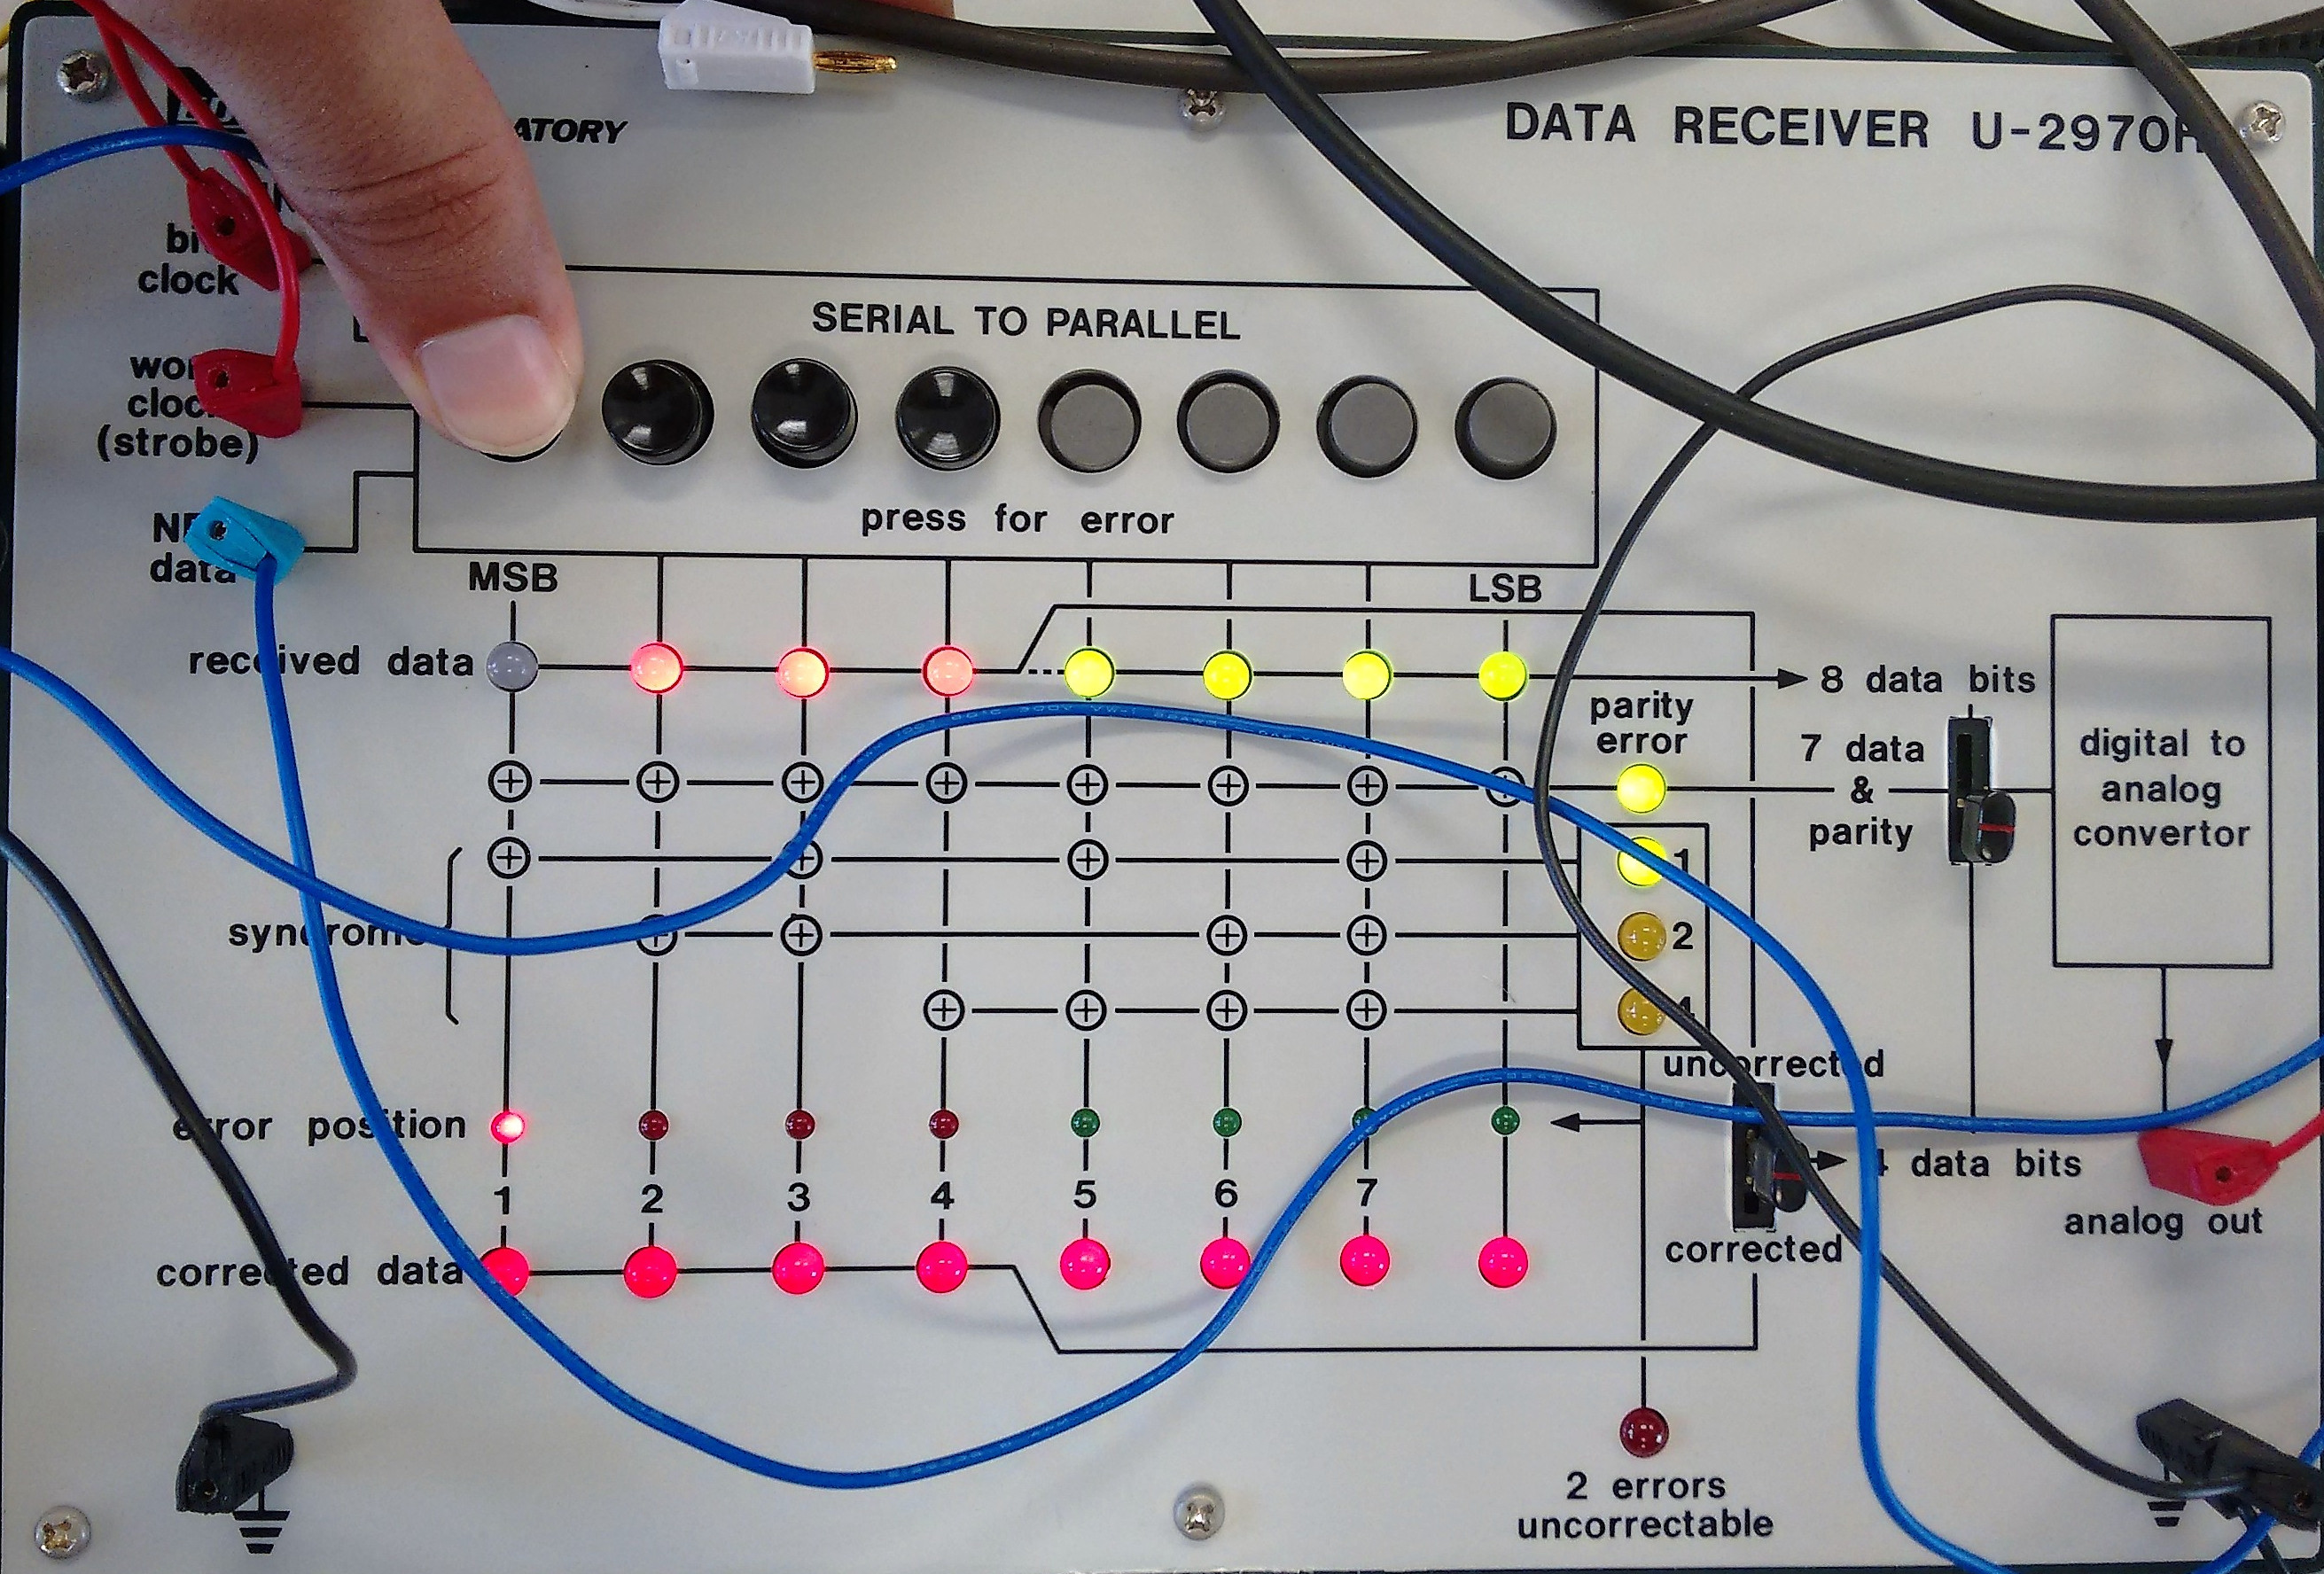
\includegraphics[scale=0.1]{r10a}
         
         \label{fig:r10a}
        \end{figure} 
        
    \subsection{Método para regeneração do clock}
    As figuras \ref{fig:r11a}, \ref{fig:r11a-2}, \ref{fig:r11a-3}, \ref{fig:r11a-4}, \ref{fig:r11a-5} e \ref{fig:r11a-6} mostram como ficou a montagem, enquanto a figura \ref{fig:r11a-7} mostra os sinais de sincronismo obtidos no osciloscópio. 
    
         \begin{figure}[H]
             \centering
             \caption{Montagem parte 11.}
             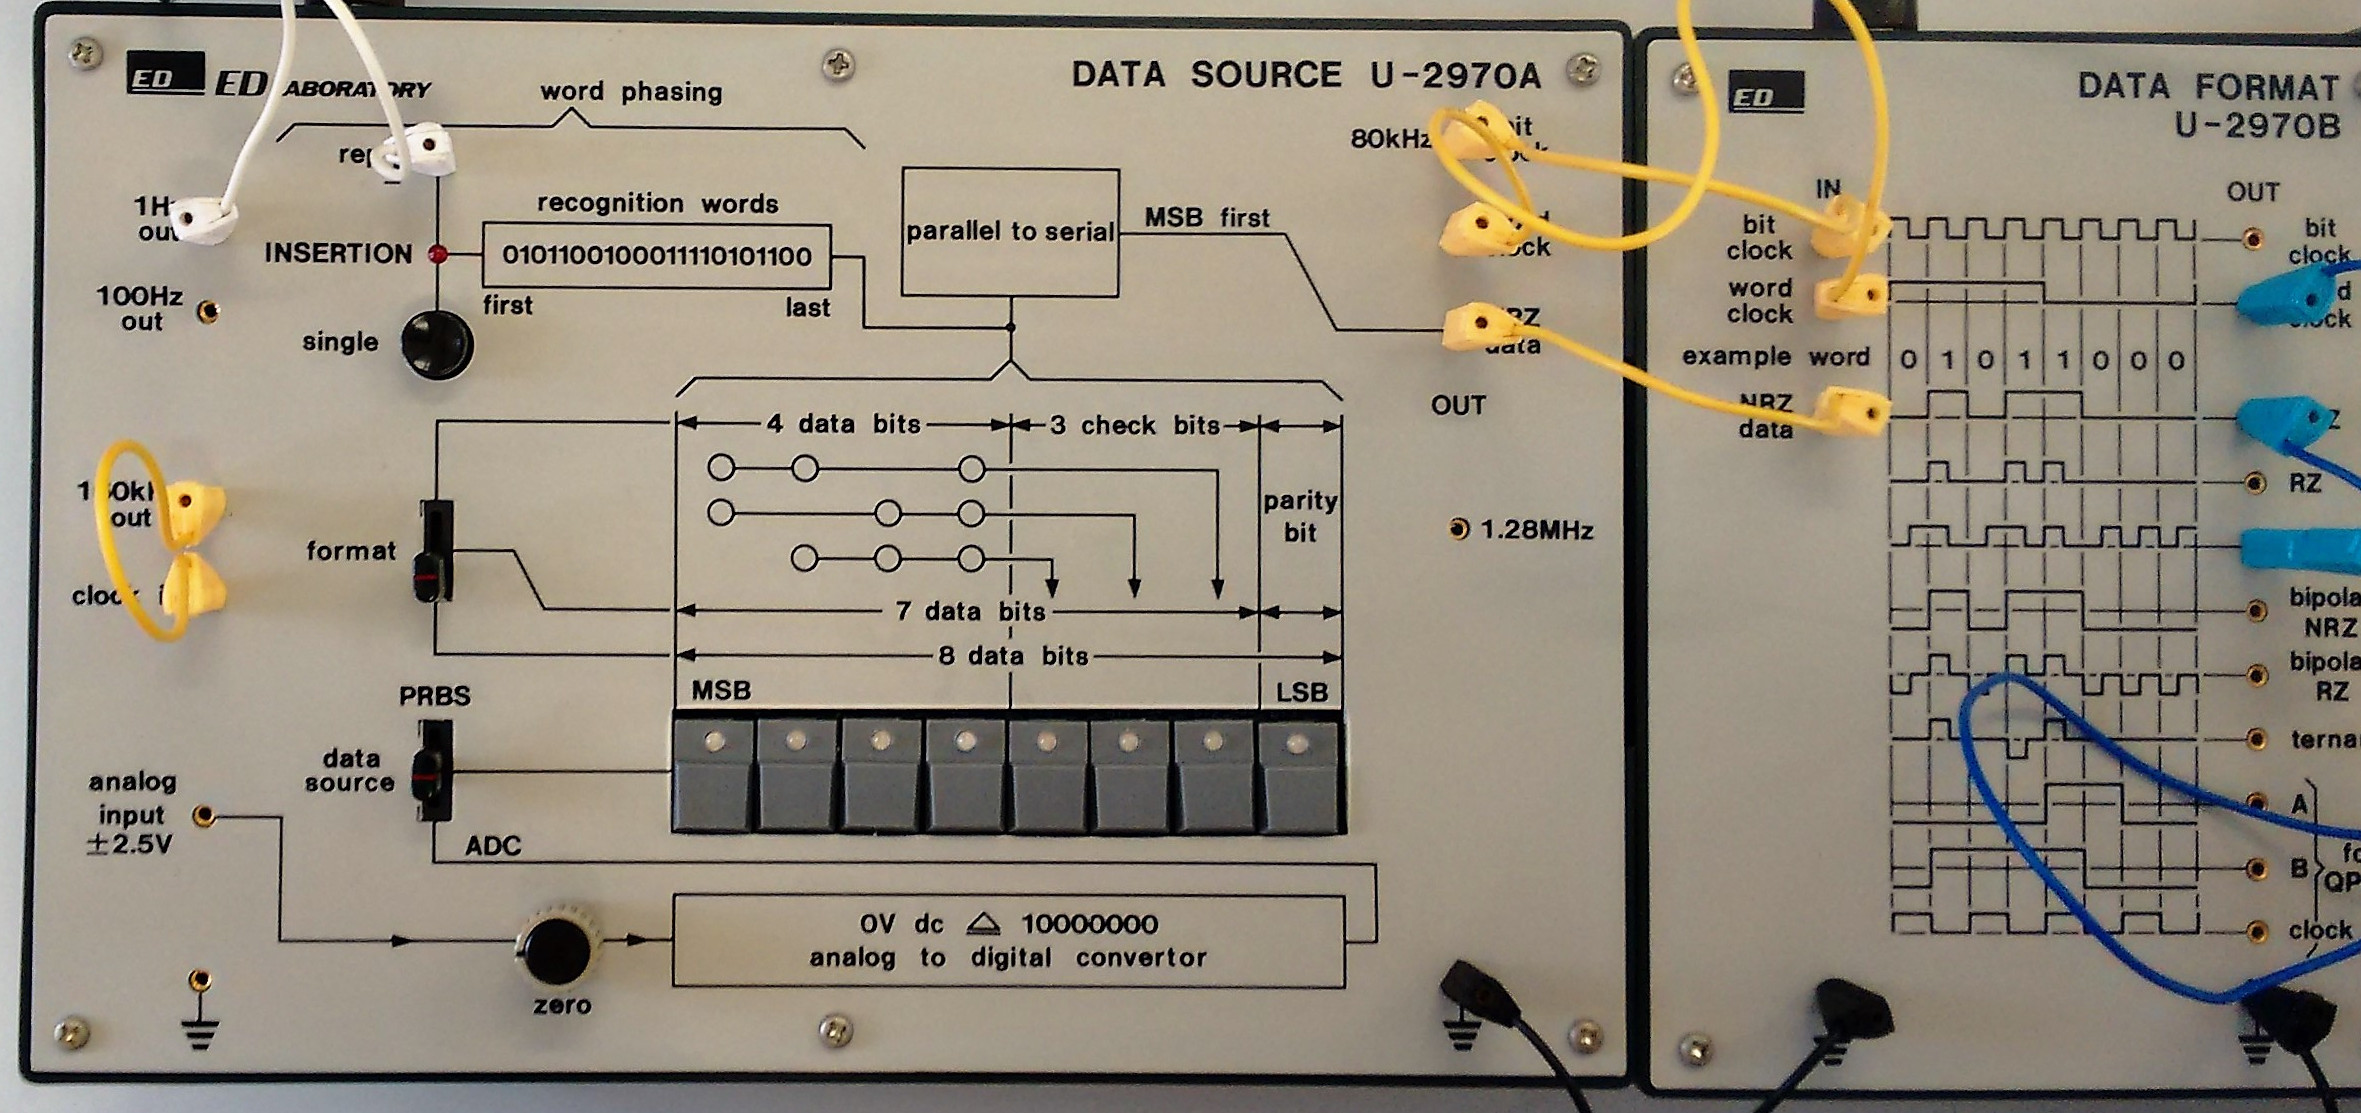
\includegraphics[scale=0.1]{r11a}
             
             \label{fig:r11a}
            \end{figure} 
           \begin{figure}[H]
               \centering
               \caption{Montagem parte 11.}
               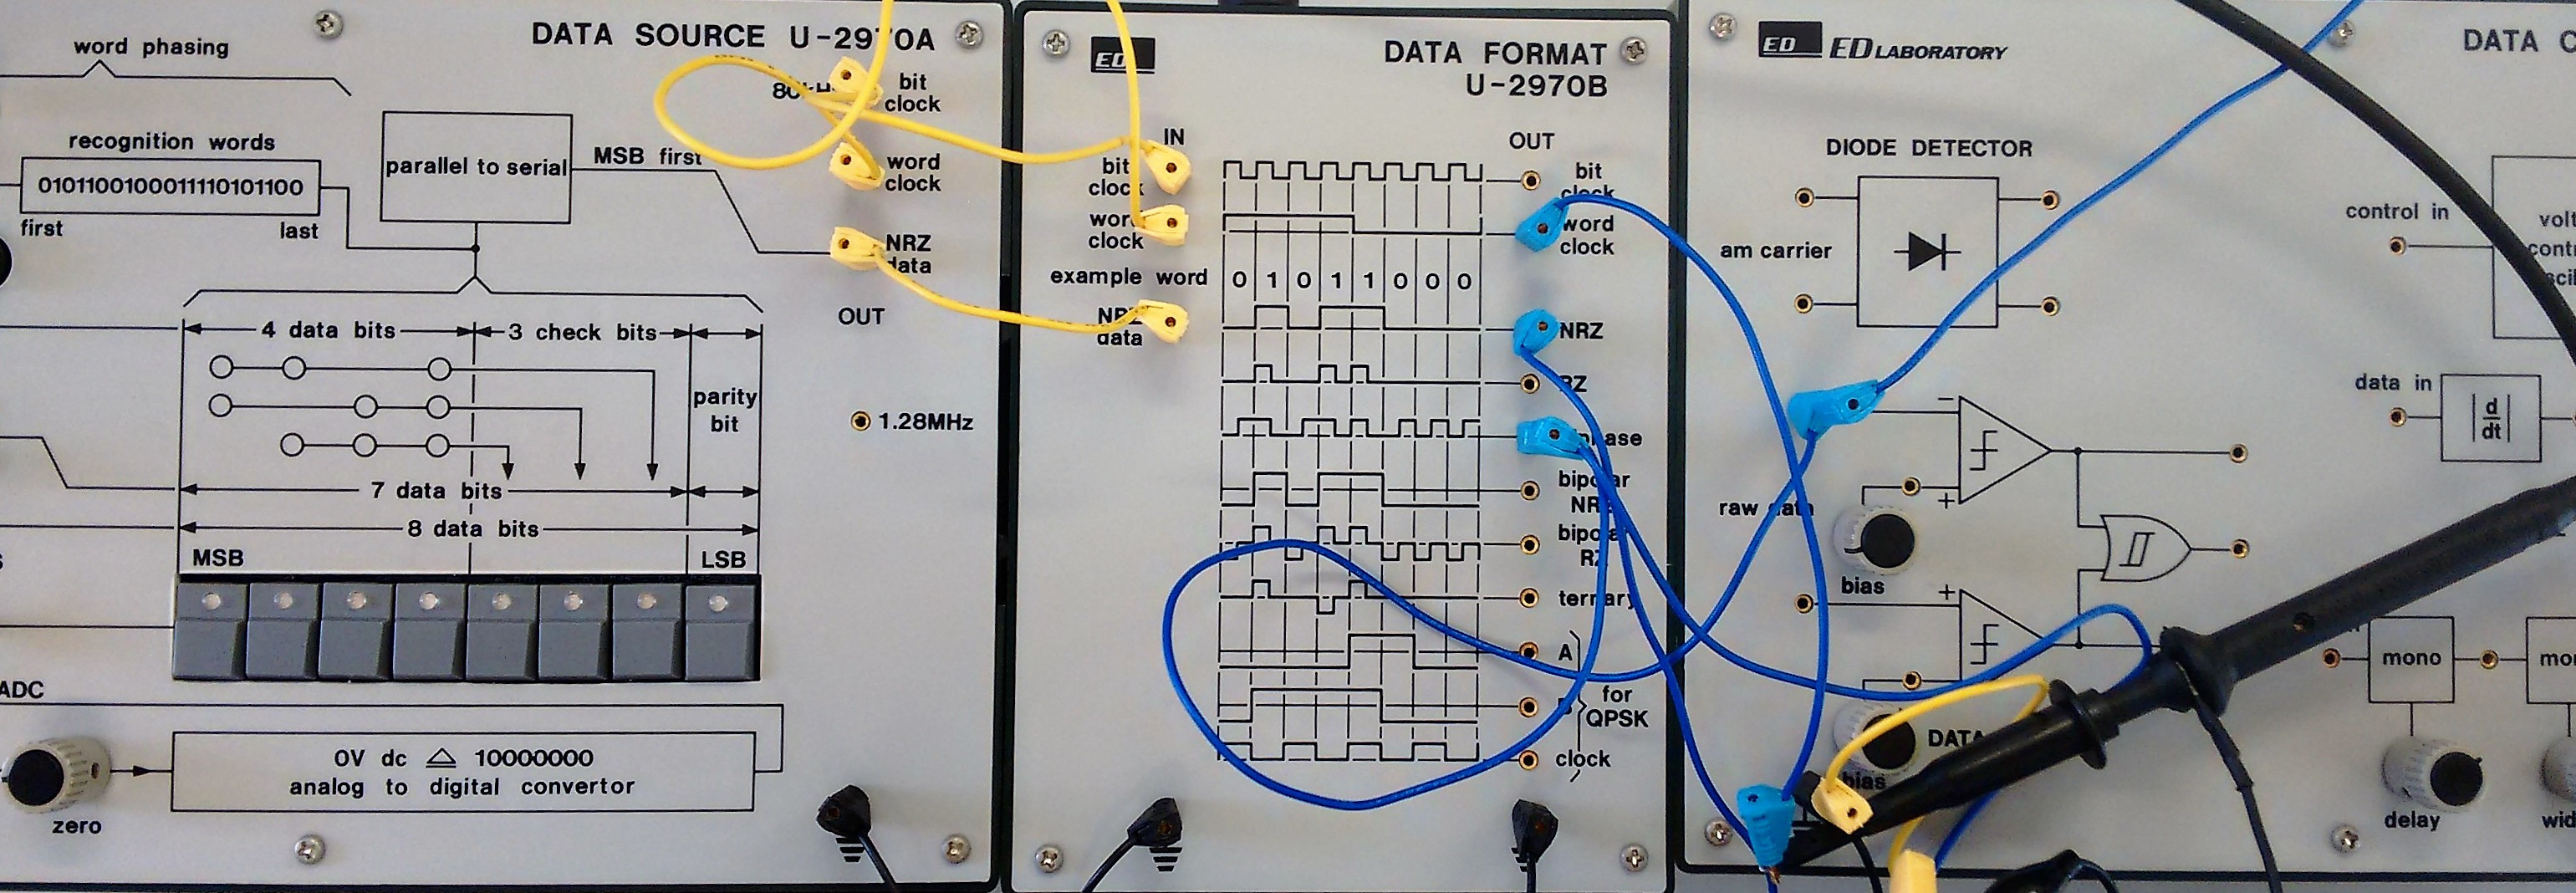
\includegraphics[scale=0.1]{r11a-2}
               
               \label{fig:r11a-2}
            \end{figure} 
        \begin{figure}[H]
            \centering
            \caption{Montagem parte 11.}
            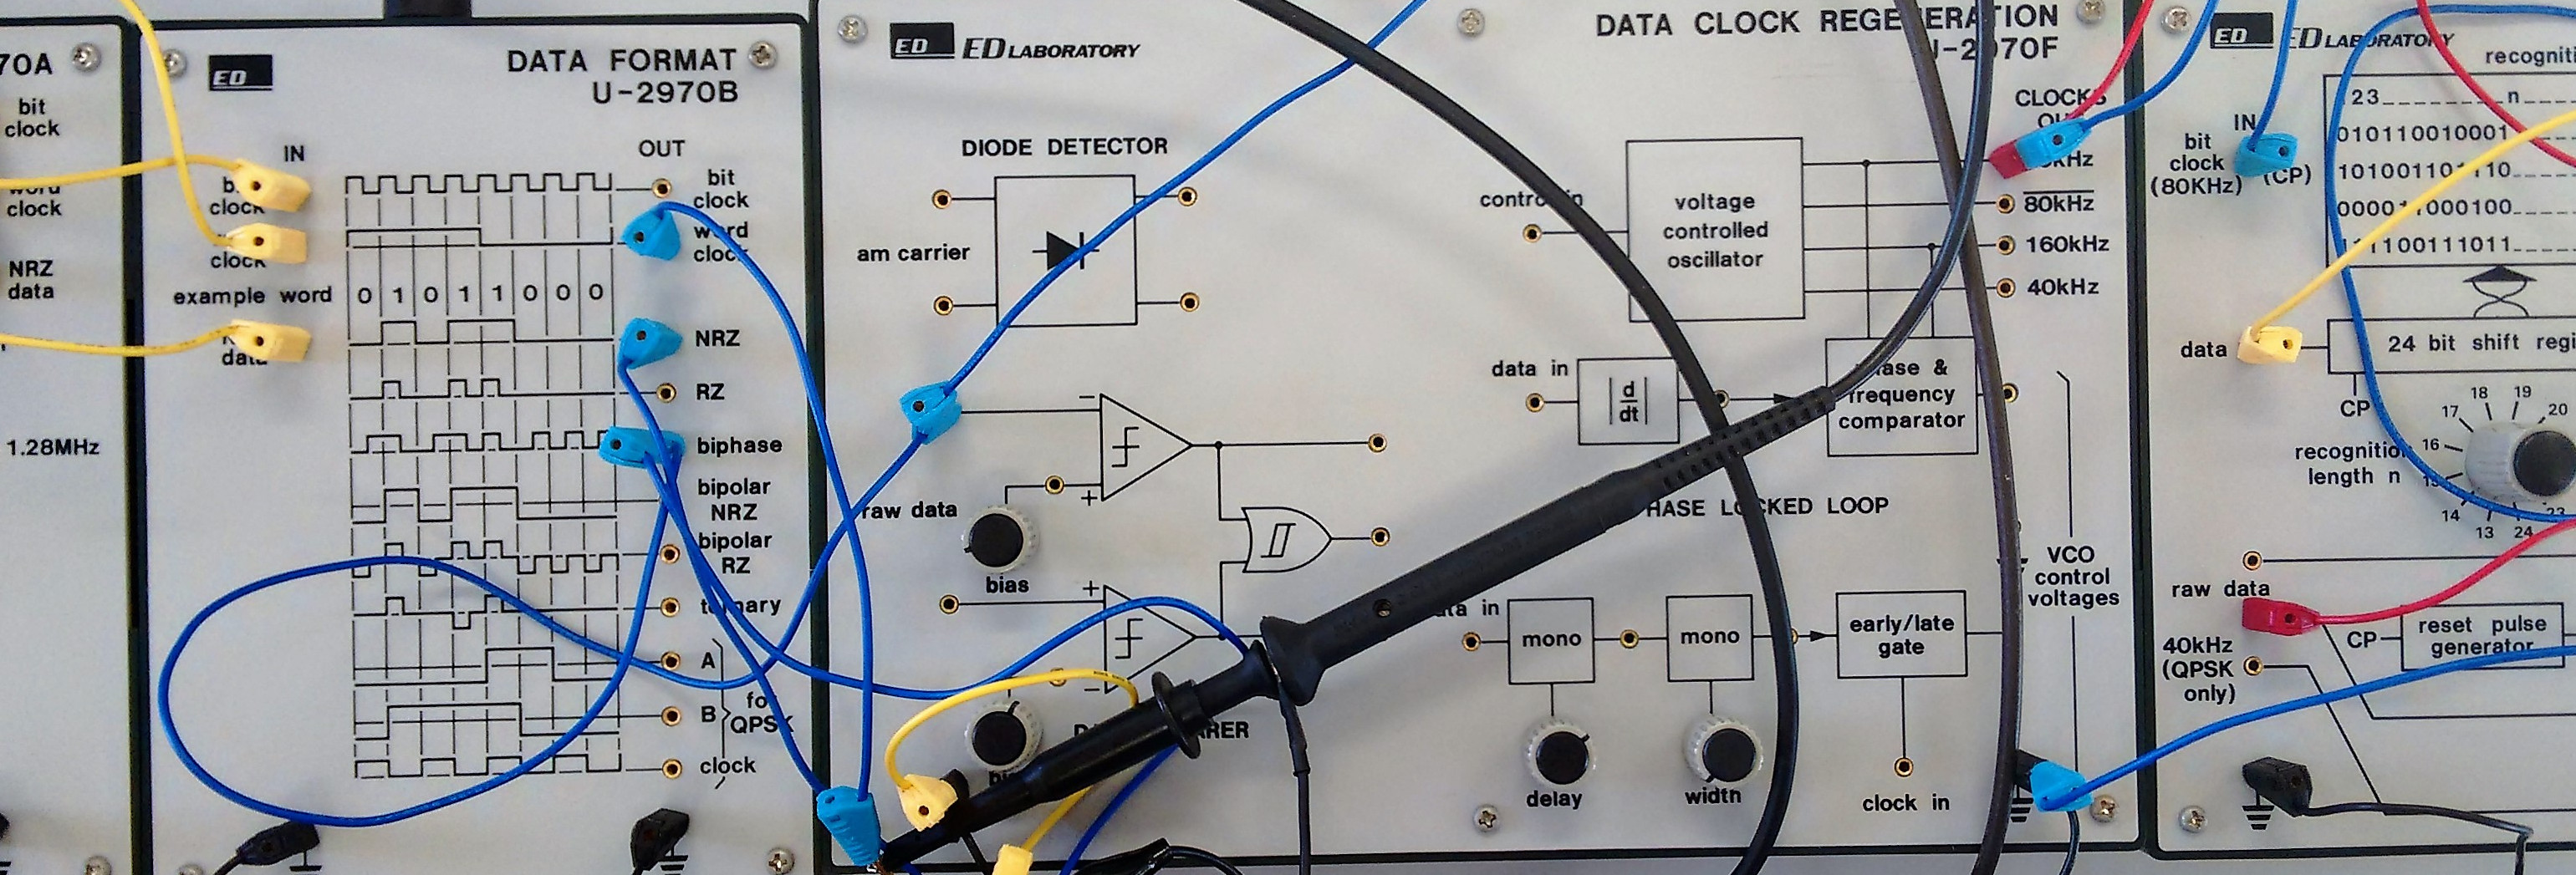
\includegraphics[scale=0.1]{r11a-3}
            
            \label{fig:r11a-3}
        \end{figure} 
        
     \begin{figure}[H]
         \centering
         \caption{Montagem parte 11.}
         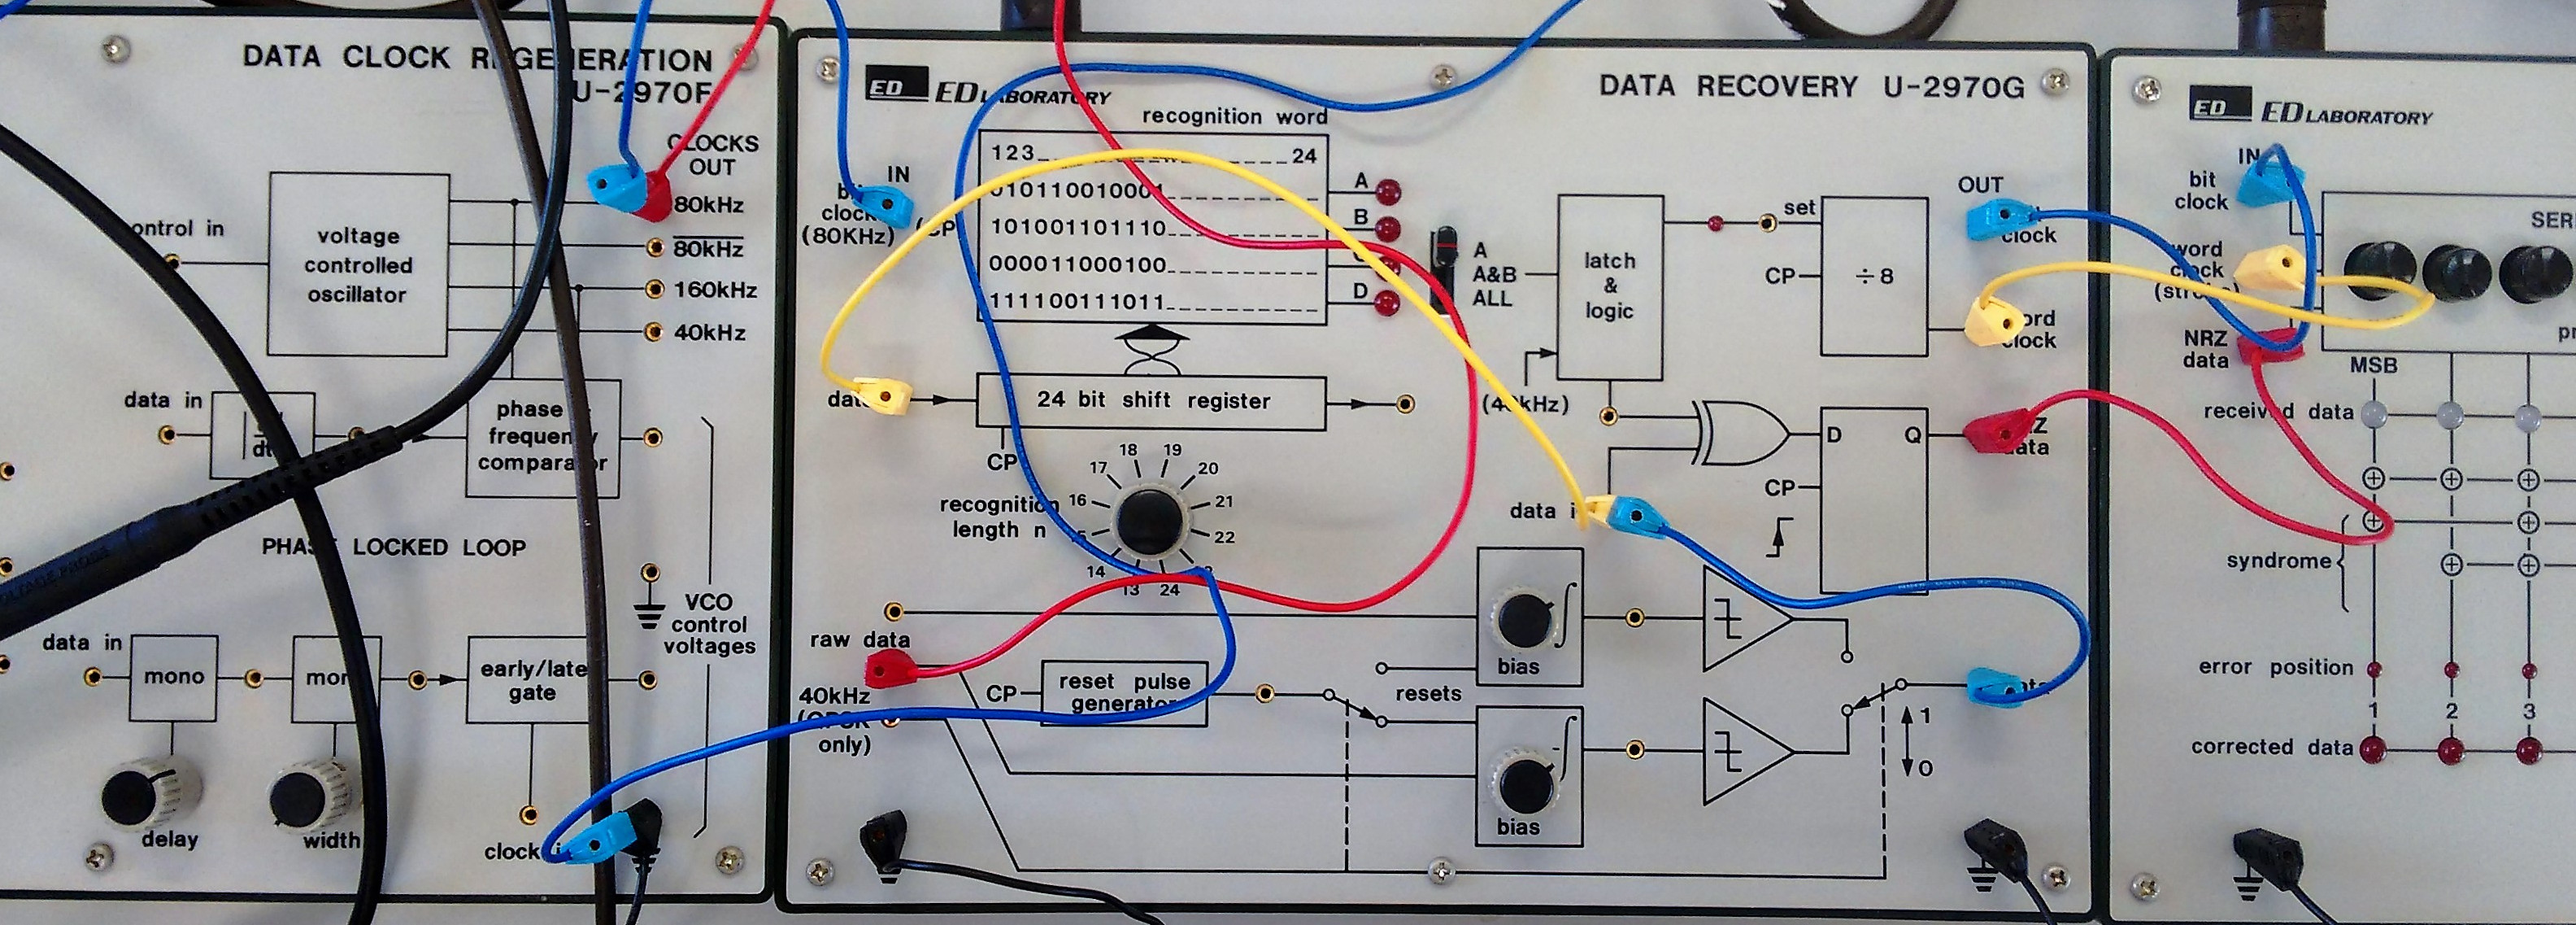
\includegraphics[scale=0.1]{r11a-4}
         
         \label{fig:r11a-4}
        \end{figure} 
     \begin{figure}[H]
         \centering
         \caption{Montagem parte 11.}
         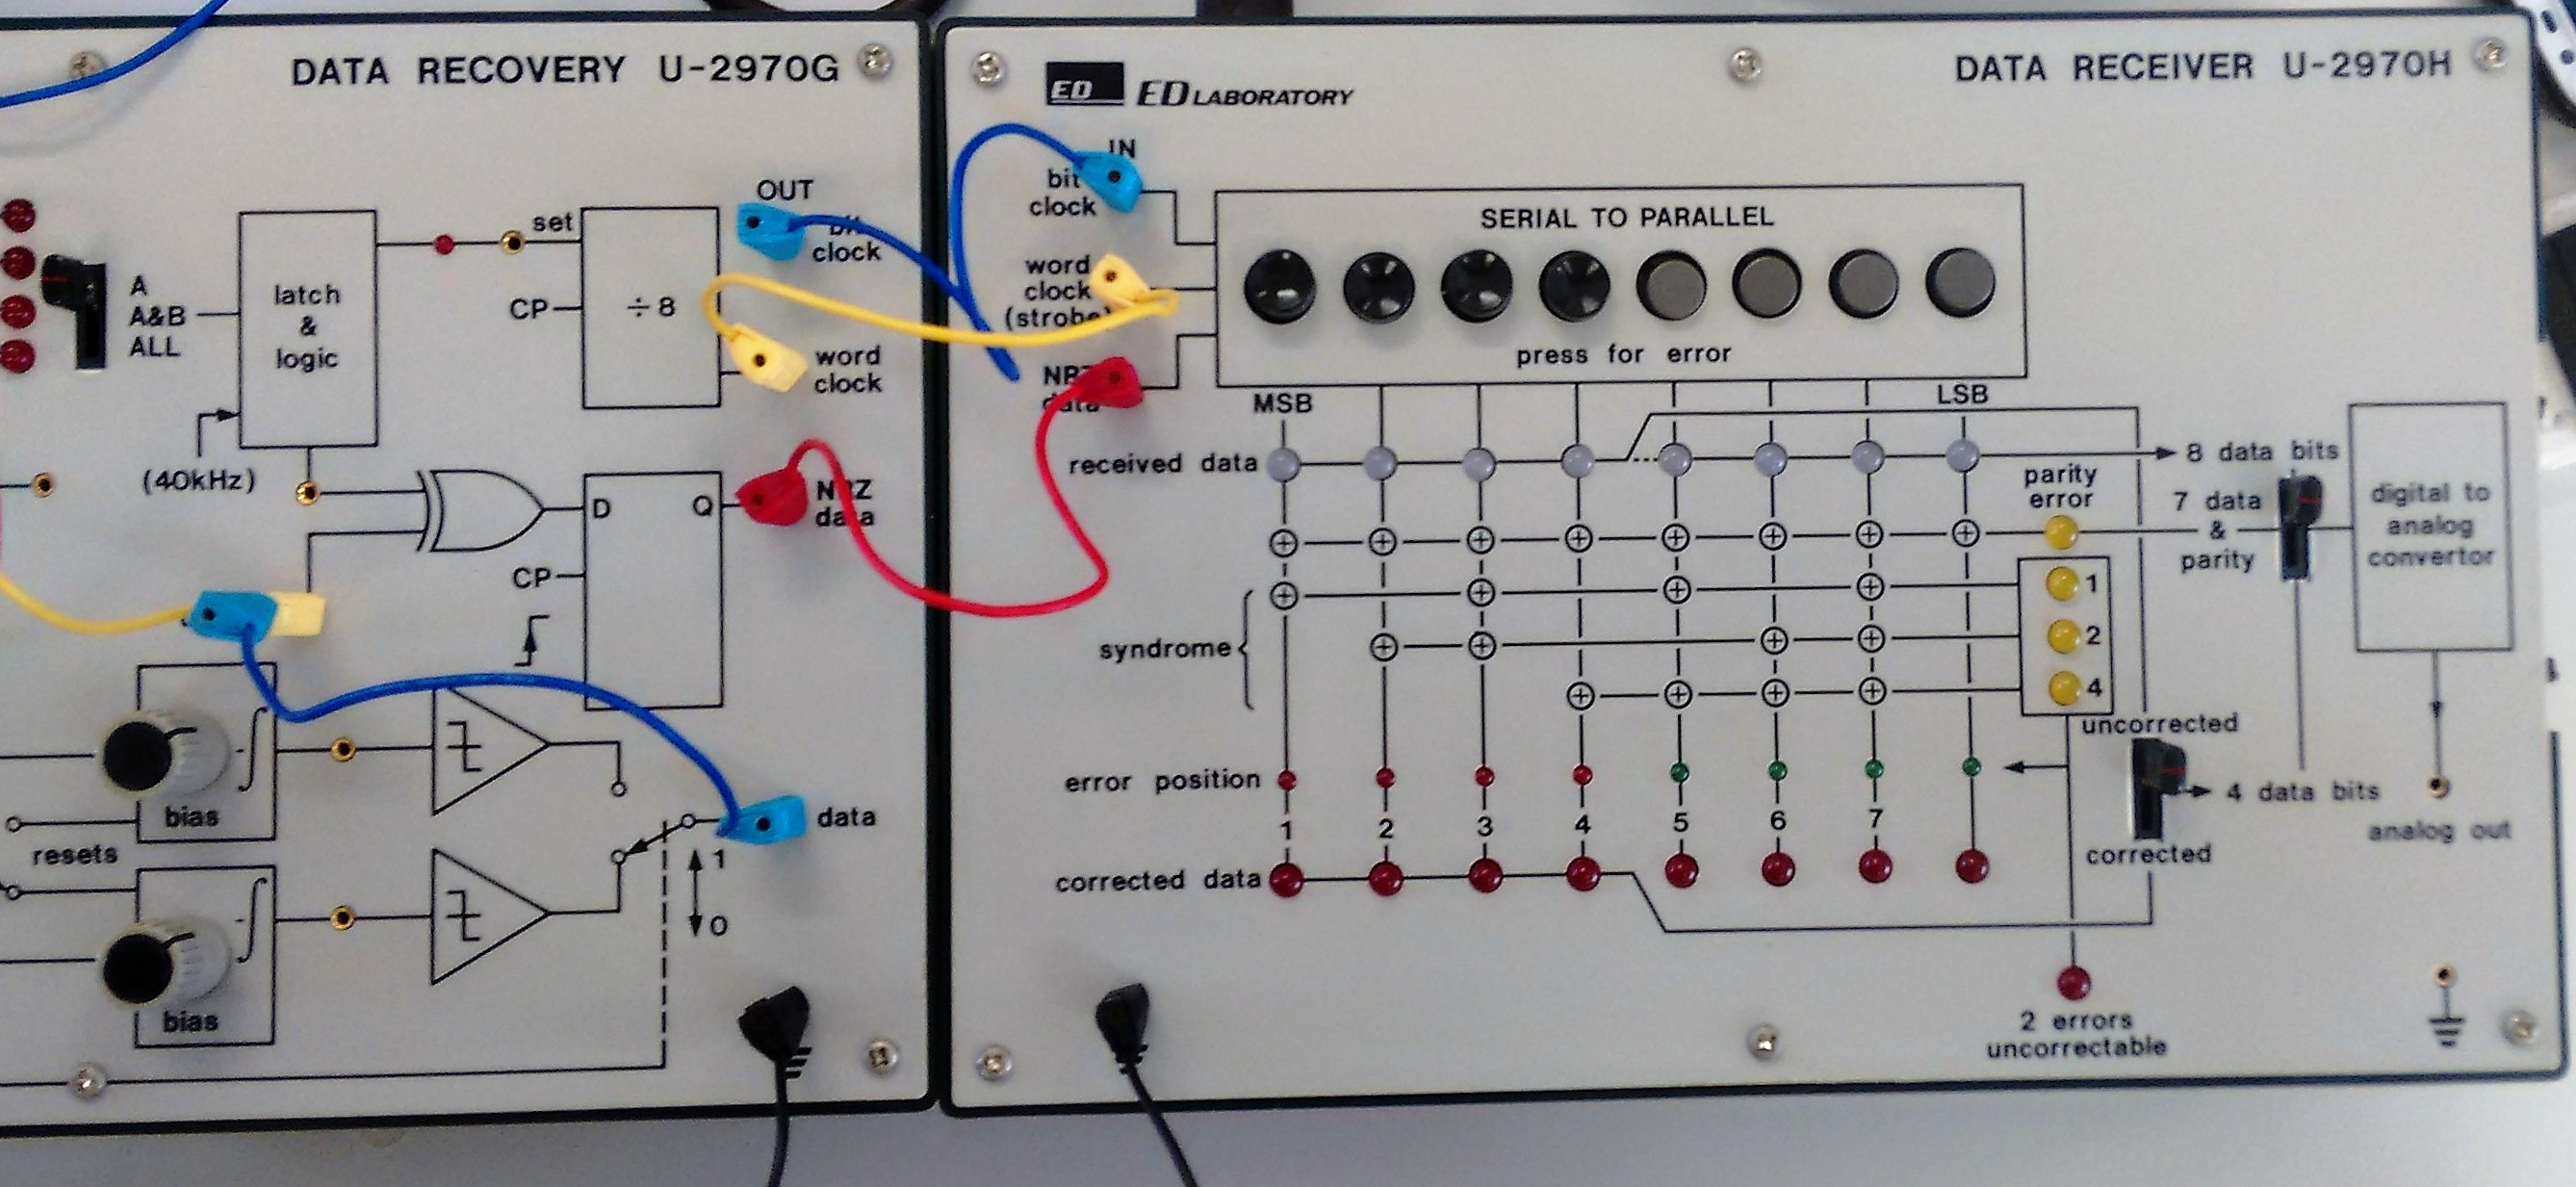
\includegraphics[scale=0.1]{r11a-5}
         
         \label{fig:r11a-5}
        \end{figure} 

\begin{figure}[H]        
         \centering        
         \caption{Montagem parte 11.}       
         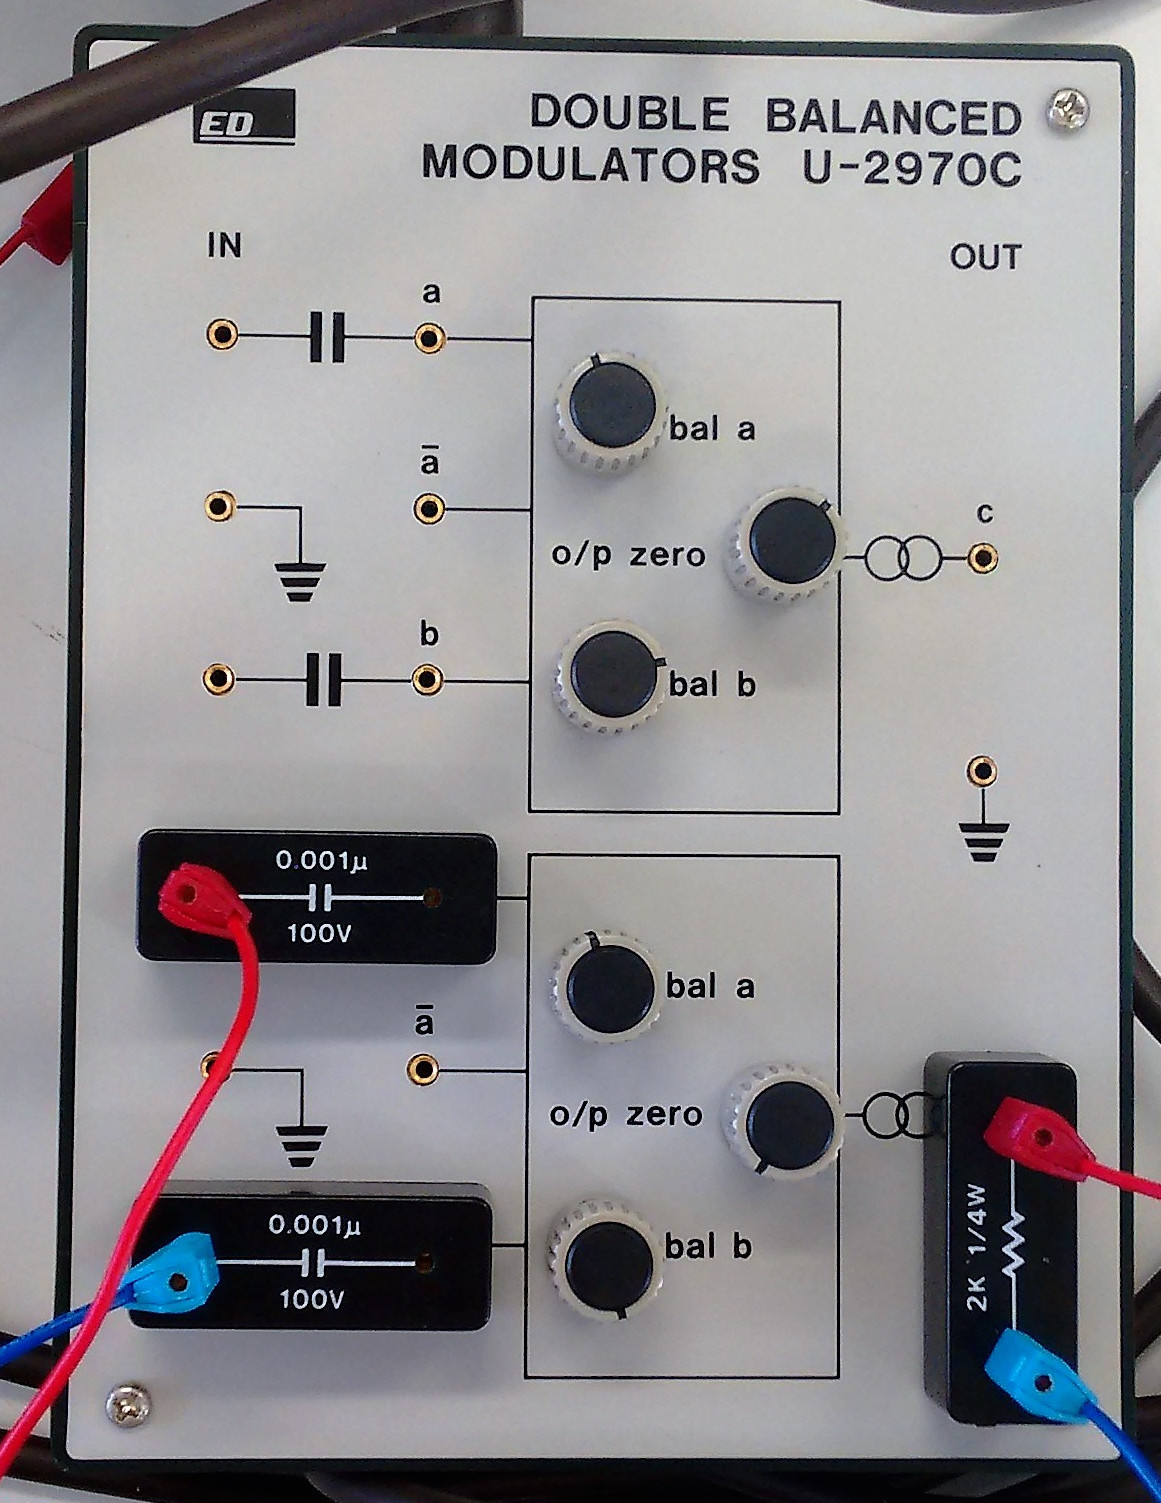
\includegraphics[scale=0.1]{r11a-6}    
         
         \label{fig:r11a-6}
        \end{figure}
\begin{figure}[H]        
    \centering        
    \caption{Saída parte 11.}       
    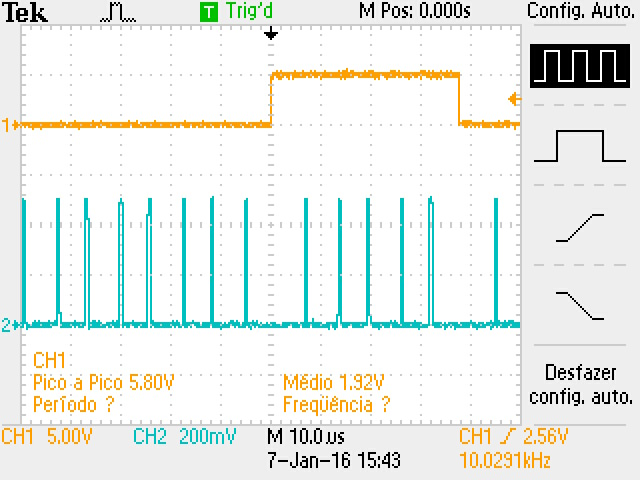
\includegraphics[scale=0.3]{r11a-7}    
    
    \label{fig:r11a-7}
\end{figure}

\subsection{Recuperação dos dados - INTEGRATE-AND-DUMP}
    A saída obtida na recuperação dos dados é mostrada na figura \ref{fig:r12a}, onde é possível observar claramente o atraso de 1 bit, devido ao integrador.
    
    Já a figura \ref{fig:r12a-2} mostra os dados recebidos em comparação com a entrada.
    
\begin{figure}[H]        
    \centering        
    \caption{Saída parte 12.}       
    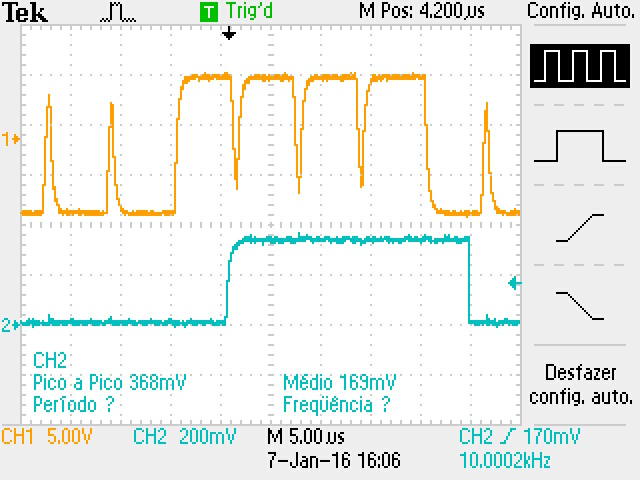
\includegraphics[scale=0.3]{r12a}    
    
    \label{fig:r12a}
\end{figure}    


\begin{figure}[H]        
    \centering        
    \caption{Saída parte 12.}       
    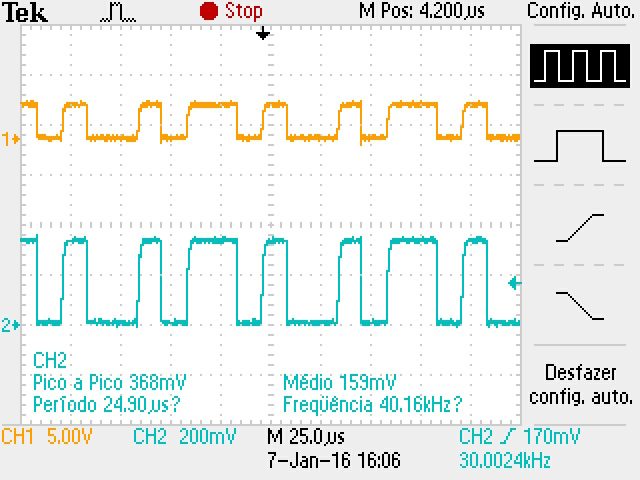
\includegraphics[scale=0.3]{r12a-2}    
    
    \label{fig:r12a-2}
\end{figure}    
    
